\documentclass[11pt,a4paper]{book}

\usepackage[utf8]{inputenc}
\usepackage[spanish]{babel}
\usepackage{latexsym}

\usepackage{amsfonts}
\usepackage[leqno]{amsmath}
\usepackage{rotating}
\usepackage{url}
\usepackage{proof}
\usepackage{alltt}
\usepackage{hyperref}
\usepackage{verbatim}
\usepackage{amssymb}

\usepackage{graphicx}
\usepackage[usenames]{color}
\usepackage{psfrag}
\usepackage{xypic}
\usepackage{proof}
\usepackage{indentfirst}
\usepackage[verbose]{geometry}
\usepackage{appendix}
\geometry{a4paper}
\geometry{top=3cm,bottom=3cm,left=3cm,right=3cm,headsep=1cm}

% oooooooooooooooooooooooooooooooooooooooooooooooooooooooooo
\makeatletter
\def\es@decimal{{.}}
\makeatother

\usepackage{pdfpages}
\usepackage{fancyhdr}
\renewcommand{\labelitemi}{\leavevmode\hbox to 1.2ex
      {\hss\vrule height .9ex width .7ex depth -.2ex\hss}}
\pagestyle{fancy}
  \renewcommand{\headrulewidth}{0pt}

\renewcommand{\chaptermark}[1]{\markboth{\chaptername\ \thechapter.\ #1}{}}
\renewcommand{\sectionmark}[1]{\markright{\thesection.\ #1}}

\fancyhf{}
\fancyhead[LO]{\textsc{\rightmark}}
\fancyhead[RE]{\textsc{\leftmark}}
\fancyhead[RO,LE]{\thepage}
\fancyfoot[LE,RO]{}
\fancypagestyle{plain}{%
  \fancyhf{}  
  \fancyfoot[C]{\thepage}
  \renewcommand{\headrulewidth}{0pt}
}


 \newtheorem{prop}{Proposition}[section]
 \newtheorem{theo}{Theorem}[section]
 \newtheorem{lemma}{Lemma}[section]
 \newtheorem{constr}{Construction}[section]
 \newtheorem{defin}{Definition}[section]
 \newtheorem{ex}{Example}[section]
 \newtheorem{alg}{Algorithm}[section]
      \newtheorem{cor}{Corollary}[section]
 \newtheorem{pro}{Problem}[section]
\newtheorem{COROLLARY}{\indent Corollary}
\newenvironment{corollary}[1]
{\begin{COROLLARY}\fullstop\label{#1}\sl}{\rm\end{COROLLARY}}
\newtheorem{EXAMPLE}{\indent Example}
\newenvironment{example}[1]
{\begin{EXAMPLE}\fullstop\label{#1}\rm}{\rm\end{EXAMPLE}}
\newtheorem{THEOREM}{\indent Theorem}
\newenvironment{theorem}[1]
{\begin{THEOREM}\fullstop\label{#1}\sl}{\rm\end{THEOREM}}
\newtheorem{REMARK}{\indent Remark}
\newenvironment{remark}[1]
{\begin{REMARK}\fullstop\label{#1}\rm}{\rm\end{REMARK}}
\newcommand{\bldu}{{\bf u}}
\newcommand{\bldv}{{\bf v}}
\newcommand{\bldy}{{\bf y}}
\newcommand{\ontopof}[2]{{{\scriptstyle{#1}} \atop {\scriptstyle{#2}}}}
\newcommand{\Eq}[1]{(\ref{#1})}
\newcommand{\bldalpha}{\mbox{\boldmath $\alpha$}}
\newcommand{\be}{\mbox{$\beta$}}
\newcommand{\clauseend}{\hspace*{\fill}\mbox{$\bullet$}}
\newcommand{\fullstop}{\hspace{-0.85em} {\bf .}}
\newcommand{\bldc}{{\bf c}}
\newcommand{\deff}{\stackrel{\Delta}{=}}
\newcommand{\ur}{\mbox{$\underline{r}$}}
\newcommand{\ua}{\mbox{$\underline{a}$}}
\newcommand{\ub}{\mbox{$\underline{b}$}}
\newcommand{\uh}{\mbox{$\underline{h}$}}
\newcommand{\uv}{\mbox{$\underline{v}$}}
\newcommand{\ue}{\mbox{$\underline{e}$}}
\newcommand{\us}{\mbox{$\underline{s}$}}
\newcommand{\uu}{\mbox{$\underline{u}$}}
\newcommand{\uy}{\mbox{$\underline{y}$}}
\newcommand{\ux}{\mbox{$\underline{x}$}}
\newcommand{\uc}{\mbox{$\underline{c}$}}
\newcommand{\ud}{\mbox{$\underline{d}$}}
\newcommand{\ut}{\mbox{$\underline{t}$}}
\newcommand{\ug}{\mbox{$\underline{g}$}}
\newcommand{\hX}{\mbox{$\hat{X}$}}
\newcommand{\hY}{\mbox{$\hat{Y}$}}
\newcommand{\hZ}{\mbox{$\hat{Z}$}}
\newcommand{\hs}{\mbox{$\hat{s}$}}
\newcommand{\hS}{\mbox{$\hat{S}$}}
\newcommand{\ra}{\mbox{$\rightarrow$}}
\newcommand{\Ra}{\mbox{$\Rightarrow$}}
\newcommand{\La}{\mbox{$\Leftarrow$}}
\newcommand{\la}{\mbox{$\leftarrow$}}
\newcommand{\lra}{\mbox{$\leftrightarrow$}}
\newcommand{\lam}{\mbox{$\lambda$}}
\newcommand{\al}{\mbox{$\alpha$}}
%\newcommand{\r}{\mbox{$\rho$}}
\newcommand{\si}{\mbox{$\sigma$}}
\newcommand{\eq}{\mbox{$\, =\,$}}
\newcommand{\om}{\mbox{$\omega$}}
\newcommand{\lan}{\mbox{$\langle$}}
\newcommand{\ran}{\mbox{$\rangle$}}
\newcommand{\lf}{\mbox{$\lfloor$}}
\newcommand{\rf}{\mbox{$\rfloor$}}
\newcommand{\lc}{\mbox{$\lceil$}}
\newcommand{\rc}{\mbox{$\rceil$}}
\newcommand{\ap}{\mbox{$\approx$}}
\newcommand{\qed}{\hfill$\Box$\\[1ex]}
\newcommand{\pf}{{\bf Proof: }}
\newcommand{\pr}{\vspace{.8cm} {\bf Problems}}
\newcommand{\uw}{\mbox{$\underline{w}$}}
\newcommand{\uell}{\mbox{$\underline{\ell}$}}
\newcommand{\uzero}{\mbox{$\underline{0}$}}
\newcommand{\uone}{\mbox{$\underline{1}$}}
\newcommand{\xor}{\mbox{$\oplus$}}
\newcommand{\lcm}{\mbox{${\rm lcm}$}}
\newcommand{\C}{\mbox{${\cal C}$}}
\newcommand{\B}{\mbox{${\cal B}$}}
\newcommand{\hU}{\mbox{${\hat{U}}$}}
\newcommand{\hV}{\mbox{${\hat{V}}$}}
\newcommand{\hW}{\mbox{${\hat{W}}$}}
\newcommand{\hA}{\mbox{${\hat{A}}$}}
\newcommand{\s}{\mbox{${\cal S}$}}
\newcommand{\A}{\mbox{${\cal A}$}}
\newcommand{\EO}{\mbox{${\cal EO}$}}
\newcommand{\E}{\mbox{${\cal E}$}}
\newcommand{\R}{\mbox{${\cal R}$}}
\newcommand{\G}{\mbox{${\cal G}$}}
\newcommand{\cC}{\mbox{${\cal C}$}}
\newcommand{\cO}{\mbox{${\cal O}$}}
\newcommand{\rg}{\mbox{$\overrightarrow{g}$}}
\newcommand{\lag}{\mbox{$\overleftarrow{g}$}}
\newcommand{\dummy}{\mbox{$\,$}}
\newcommand{\bp}{\newpage}
\newcommand{\br}{\\ }
\newcommand{\ce}{\begin{center}}
\newcommand{\cen}{\end{center}}
\newcommand{\fB}{\bf}
\newcommand{\fI}{\it}
\newcommand{\fR}{\rm}
\newcommand{\hl}{\dummy\hrulefill\dummy}
\newcommand{\ip}[1]{\item[{\rm {#1}}]}
\newcommand{\ipb}{\begin{description}}
\newcommand{\ipn}{\end{description}}
\newcommand{\lp}{\par\noindent}
\newcommand{\bld}[1]{{\bf {#1}}}
\newcommand{\itl}[1]{{\it {#1}}}
\newcommand{\rmn}[1]{{\rm {#1}}}
\newcommand{\pp}{\par}
\newcommand{\qb}{\begin{quote}}
\newcommand{\qn}{\end{quote}}
\newcommand{\sh}[2]{\section{\Pd #1}\label{#2}}
\newcommand{\spc}[1]{\vspace{#1}}
\newcommand{\tp}{\begin{titlepage}}
\newcommand{\tpn}{\end{titlepage}}
\newcommand{\zb}{\begin{figure}[hbtp]}
\newcommand{\zn}{\end{figure}}
\newcommand{\EQ}{\[}
\newcommand{\EN}{\]}
\newcommand{\EQX}[1]{\begin{equation}\label{#1}}
\newcommand{\ENX}{\end{equation}}
\newcommand{\EQL}{\begin{eqnarray*}}
\newcommand{\ENL}{\end{eqnarray*}}
\newcommand{\EQLX}[1]{\begin{eqnarray}\label{#1}}
\newcommand{\ENLX}{\end{eqnarray}}
\newcommand{\Pd}{\hspace{-1.35em}
           {\bf .} \hspace {0.35em}}
\newcommand{\lpsh}{\nopagebreak\par\noindent\nopagebreak}
\newcommand{\ppsh}{\nopagebreak\par\nopagebreak}
\newcommand{\open}{\begin{document}}
\newcommand{\close}{\end{document}}
\newcommand{\lfcr}[1]{\br\hspace*{#1em}}
\newenvironment{mat}[1]
{\left[\begin{array}{#1}}{\end{array}\right]}
\newcommand{\GAMMA}{\Gamma}
\newcommand{\DELTA}{\Delta}
\newcommand{\THETA}{\Theta}
\newcommand{\LAMBDA}{\Lambda}
\newcommand{\XI}{\Xi}
\newcommand{\PI}{\Pi}
\newcommand{\SIGMA}{\Sigma}
\newcommand{\UPSILON}{\Upsilon}
\newcommand{\PHI}{\Phi}
\newcommand{\PSI}{\Psi}
\newcommand{\OMEGA}{\Omega}
\newcommand{\bldgreek}[1]{\mbox{\boldmath $#1$}}
\newcommand{\bldbeta}{\bldgreek{\beta}}
\newcommand{\bldgamma}{\bldgreek{\gamma}}
\newcommand{\blddelta}{\bldgreek{\delta}}
\newcommand{\bldepsilon}{\bldgreek{\epsilon}}
\newcommand{\bldvarepsilon}{\bldgreek{\varepsilon}}
\newcommand{\bldzeta}{\bldgreek{\zeta}}
\newcommand{\bldeta}{\bldgreek{\eta}}
\newcommand{\bldtheta}{\bldgreek{\theta}}
\newcommand{\bldvartheta}{\bldgreek{\vartheta}}
\newcommand{\bldiota}{\bldgreek{\iota}}
\newcommand{\bldkappa}{\bldgreek{\kappa}}
\newcommand{\bldlambda}{\bldgreek{\lambda}}
\newcommand{\bldmu}{\bldgreek{\mu}}
\newcommand{\bldnu}{\bldgreek{\nu}}
\newcommand{\bldxi}{\bldgreek{\xi}}
\newcommand{\bldpi}{\bldgreek{\pi}}
\newcommand{\bldvarpi}{\bldgreek{\varpi}}
\newcommand{\bldrho}{\bldgreek{\rho}}
\newcommand{\bldvarrho}{\bldgreek{\varrho}}
\newcommand{\bldsigma}{\bldgreek{\sigma}}
\newcommand{\bldvarsigma}{\bldgreek{\varsigma}}
\newcommand{\bldtau}{\bldgreek{\tau}}
\newcommand{\bldupsilon}{\bldgreek{\upsilon}}
\newcommand{\bldphi}{\bldgreek{\phi}}
\newcommand{\bldvarphi}{\bldgreek{\varphi}}
\newcommand{\bldchi}{\bldgreek{\chi}}
\newcommand{\bldpsi}{\bldgreek{\psi}}
\newcommand{\bldomega}{\bldgreek{\omega}}
\addto\extrasspanish{\def\tablename{Tabla}}

% oooooooooooooooooooooooooooooooooooooooooooooooooooooooooo

\graphicspath{{images/}}
\begin{document}

\begin{frontmatter}

\thispagestyle{empty}

\begin{huge}
\mbox{ }
\vfill
\newlength{\longTitulo}
\begin{center}

\rule{145mm}{.5mm}\\
\vskip .3cm
\textbf{VNC++, control remoto desde Android}\\
\rule{145mm}{.5mm}\\

\end{center}
\end{huge}

\vfill


  \begin{center}
				{\scalebox{.3}{
\includegraphics{LogoUCM}}}
  \end{center}

\vfill

\begin{center}
  {\Large {\bf TRABAJO FIN DE GRADO}}
\end{center}

\begin{center}
  {\Large {\bf CURSO 2012-2013}}
\end{center}

\vfill


\begin{large}
\begin{center}
\begin{large}
  	{\bf \'Oscar Crespo Salazar}\\
	{\bf Gorka Jimeno Garrach\'on}\\
	{\bf Luis Valero Mart\'in}
\end{large}
  \\ \mbox{ } \\ \mbox{ } \\ 
{\it Director}  \\ [0.3em]
  {\bf  Antonio Sarasa Cabezuelo}
  \vspace{.5ex}
\begin{large}
\begin{center}
\vspace{3ex}
\text{Departamento de Sistemas Inform\'aticos y Computaci\'on}\\[0.2em]
\text{Facultad de Inform\'atica}\\[0.2em]
\text{Universidad Complutense de Madrid}\\[1em]
\text{Madrid, Junio de 2013}
\end{center}
\end{large}
\end{center}

\vfill

\end{large}

\newpage
\thispagestyle{empty}
\mbox{ }


\clearpage
\pagestyle{fancy}
\fancyhf{}
\fancyhead[LO]{\textsc{\rightmark}}
\fancyhead[RE]{\textsc{\leftmark}}
\fancyhead[RO,LE]{\thepage}
\fancyfoot[LE,RO]{}
\fancypagestyle{plain}{
  \fancyhf{}  
  \fancyfoot[C]{\thepage}
  \renewcommand{\headrulewidth}{0pt}
}

\end{frontmatter}


\begin{otherlanguage}{spanish}
\section*{Licencias}
\null
\vfill
\begin{flushleft}
\copyright 2013 All Rights Reserved.\\

\includegraphics[scale=0.15]{by-sa.png}\\
Esta obra est\'a bajo una Licencia Creative Commons Atribuci\'on-CompartirIgual 3.0 Unported.
\end{flushleft}

\newpage
\end{otherlanguage}

\newpage
\thispagestyle{empty}
\mbox{ }

\newpage

\begin{otherlanguage}{spanish}

\thispagestyle{fancy}
\section*{Agradecimientos}
Agradecemos a Johannew Shindelin por la completa librer\'ia para VNC que cre\'o y adem\'as distribuirla de forma libre. Y por supuesto por su inestimable y desinteresada ayuda en el Mailing-list de la propia librer\'ia, tanto de \'el como de Christian Beier.\\

Tambi\'en agradecer a la web stackoverflow \url{http://stackoverflow.com/}, concretamente la secci\'on de Android, por su certera ayuda con esas inevitables dudas que surgen al desarrollar c\'odigo desde cero.\\

Tambi\'en, como no, agradecer a los desarrolladores de Google, que a trav\'es de su web \url{http://developer.android.com/index.html} y ciertos ejemplos clave, han permitido culminar este proyecto.\\

Menci\'on especial para Axel Amigo, buen amigo nuestro, que nos ayud\'o poniendo voz al v\'ideo explicativo del proyecto, a Ra\'ul Crespo, por hacer el montaje que tanto nos ha satisfecho a todos, y por supuesto, a Sergio Barrasa por el fant\'astico logo realizado para la aplicaci\'on.\\

Por \'ultimo agradecer a Antonio Sarasa Cabezuelo, director del proyecto, por la confianza depositada en nosotros y su inestimable ayuda durante todo el proceso. Tambi\'en agradecemos a todos los profesores de la Facultad de Inform\'atica de la Universidad Complutense de Madrid por proporcionarnos durante todos estos años los conocimientos necesarios para que el desarrollo de este proyecto.
\end{otherlanguage}

\newpage
\thispagestyle{empty}
\mbox{ }

\newpage
%\thispagestyle{empty}
\section*{Abstract}

Nowadays there are a lot of VNC based applications for Android. Nonetheless, none of these applications are Free Software and are implemented using the NDK. The point of this project is to use the NDK potential to make a VNC based application and try to obtain a better performance than the other applications implemented using only the SDK and all the source code will be Free Software.
\\ \mbox{ } \\
\textit{\textbf{Keywords}}

VNC, Android, C++, C, NDK, SDK, JNI, RFB.


\newpage
\thispagestyle{empty}
\mbox{ }

\newpage

\begin{otherlanguage}{spanish}

\thispagestyle{fancy}
\section*{Resumen}

Hoy en día hay una gran cantidad de aplicaciones basadas en VNC para Android. Sin embargo, ninguna de estas aplicaciones son Free Software y se implementan utilizando el NDK. El objetivo de este proyecto es utilizar el potencial NDK para hacer una aplicación basada en VNC y tratar de obtener un mejor rendimiento que el resto de las aplicaciones implementadas utilizando sólo el SDK y todo el código fuente será Free Software.\\

El protocolo para comunicarse con un servidor VNC se llama RFB. Para la implementación de este protocolo en este proyecto se ha utilizado la librería libVNCServer. Esta librería facilita el control de RFB. Sin libVNCServer habría sido más difícil hacer nuestra propia librería para gestionar el protocolo. JNI se utiliza como framework para comunicar el código nativo con Java. Las tecnologías, así como el proceso utilizado para construir este software se explicará a lo largo de esta memoria. 
\\ \mbox{ } \\
\textit{\textbf{Palabras clave}}

VNC, Android, C++, C, NDK, SDK, JNI, RFB.

\end{otherlanguage}

\newpage
\thispagestyle{empty}
\mbox{ }

\newpage
\thispagestyle{empty}
\noindent Autorizamos a la Universidad Complutense de Madrid a difundir y utilizar con fines acad\'emicos, no comerciales y mencionando expresamente a sus autores, tanto la propia memoria, como el c\'odigo, los contenidos audiovisuales incluso si incluyen im\'agenes de los autores, la documentaci\'on y/o el prototipo desarrollado.\\

\vspace*{5cm}\par

\'Oscar Crespo Salazar 

\vspace*{5cm}\par 

Gorka Jimeno Garrach\'on

\vspace*{5cm}\par 

Luis Valero Mart\'in


\newpage
\thispagestyle{empty}
\mbox{ }

\newpage
\thispagestyle{empty}


\begin{otherlanguage}{spanish}

\pagestyle{empty}

\renewcommand{\contentsname}{\'Indice} 
\renewcommand{\listtablename}{\'Indice de Tablas} 
\renewcommand{\listfigurename}{\'Indice de Figuras} 
\renewcommand{\appendixname}{Ap\'endices}
\renewcommand{\appendixtocname}{Ap\'endices}
\renewcommand{\appendixpagename}{Ap\'endices}

\tableofcontents
%\listoftables
\listoffigures


\pagestyle{fancy}
\pagenumbering{arabic}

\chapter{Introducci\'on\label{ch:intro}}

El desarrollo de las redes de telecomunicaciones ha permitido que poco a poco el control remoto de un ordenador pase de meras terminales de texto a los escritorios remotos de hoy en día. La tecnología de escritorio remoto permite la centralización de aplicaciones que normalmente se ejecutarían en el entorno de usuario. Gracias a esta tecnología el entorno de usuario (cliente) se convierte en una simple terminal de entrada/salida. Todos los eventos de pulsación de teclas y movimientos del ratón se transmiten desde el cliente a un servidor donde la aplicación los procesa como si se tratasen de eventos locales. La imagen de la pantalla se devuelve al cliente y de esta manera se puede controlar desde el terminal cliente la máquina donde se encuentra la aplicación servidor.\\

Este proyecto se centra únicamente en la realización de una aplicación cliente para Android. De tal manera que la aplicación servidor queda fuera del dominio de este proyecto. Aunque más adelante se profundizará en cuales son los objetivos concretos de este proyecto, conviene aclarar que el objetivo era desarrollar un cliente VNC para Android, que utilizará el NDK y que fuera de software libre, ya que en la actualidad no existe ninguno que cumpla estos dos requisitos.\\

Existen diferentes protocolos de comunicación entre la aplicación cliente y la aplicación servidor. Este proyecto se ha desarrollado utilizando el protocolo de comunicación Remote Frame Buffer (RFB), utilizado por todos los clientes y servidores VNC. De esta manera la aplicación será compatible con cualquier servidor VNC instalado en cualquier terminal.\\

Antes de profundizar más en como se han afrontado los objetivos del proyecto conviene establecer ciertos conocimientos básicos relativos al dominio de estas aplicaciones. Comenzaremos explicando algunos conceptos que se han utilizado antes, tales como VNC, RFB, Android, etc.\\

\section{Conceptos}

\subsection{Escritorio remoto}

Un escritorio remoto es una tecnología que permite a un usuario controlar desde un terminal gráfico (cliente) otro terminal gráfico (servidor). X-Window fue el primer escritorio remoto desarrollado por el Massachusetts Institute of Technology (MIT) en la década de los ochenta.\\

\subsection{VNC}

VNC son las siglas en inglés de Virtual Network Computing. Es un sistema de escritorio remoto que utiliza el protocolo Remote Frame Buffer (RFB) para controlar remotamente otra máquina. Está basado en una arquitectura cliente-servidor, donde la máquina con la aplicación cliente es la que controla a la máquina con la aplicación servidor. VNC transmite los eventos de ratón y teclado desde el cliente al servidor y éste devuelve las actualizaciones de pantalla en la otra dirección a través de una red de comunicaciones.\\

VNC es independiente del sistema operativo, es decir, un cliente VNC ejecutado en una máquina Windows podría controlar un servidor ejecutado en una máquina Linux. En definitiva, se podría controlar cualquier sistema operativo desde cualquier sistema operativo siempre que ambos sean compatibles con VNC.\\

\subsection{RFB}

RFB son las siglas en inglés de Remote Frame Buffer. Es un protocolo de comunicación para el acceso remoto a interfaces gráficas de usuario. Como trabaja a nivel de framebuffer es aplicable a todos los sistemas de ventanas (X11, Windows, Macintosh). RFB es el protocolo usado en VNC.\\

\subsection{Android}

Android es un sistema operativo basado en Linux, diseñado principalmente para Smartphones y Tablets. Inicialmente fue desarrollado por Android Inc, pero finalmente Google lo compró en 2005. Fue presentado en 2007 junto con la fundación Open Handset Alliance y el primer móvil con sistema operativo Android salió al mercado en 2008.\\

La mayoría del código de Android está liberado bajo una licencia Apache, licencia libre y de código abierto. No obstante no está liberado completamente por lo tanto no se puede decir que Android sea un sistema operativo libre. Uno de sus puntos fuertes es la facilidad para desarrollar aplicaciones gracias a las herramientas que proporciona Google. Estas aplicaciones normalmente estan escritas en Java y se desarrollan utilizando el Android SDK, pero también se pueden construir aplicaciones escritas en C/C++ usando el Android NDK.\\

\subsection{Android SDK}

SDK son las siglas en inglés de Software Development Kit. El SDK proporcina las APIs y herramientas de desarrollo necesarias para construir, testear y depurar aplicaciones para Android.\\

\subsection{Android NDK}

NDK son las siglas en inglés de Native Development Kit. El NDK es un conjunto de herramientas que permiten desarrollar parte de la aplicación para Android con lenguajes de código nativo como C o C++.\\

\subsection{JNI}

\subsection{Tight}

\subsection{MD5}

MD5 son las siglas en inglés de Message-Digest Algorithm 5. Es un algoritmo de reducción criptográfico diseñado por el profesor Ronald Rivest del Instituto Tecnológico de Massachusetts. Es un algoritmo que para esta aplicación se ha considerado suficiente ya que es una codificación de 128 bits y todavía sigue en uso en muchos sistemas de codificación. Se descartaron sistemas más robustos como SHA-1 o SHA-2 por considerarlos demasiado pesados para una encriptación de este tipo.

\subsection{Free Software}

\subsection{GPL}

\section{Motivaciones}

La motivación principal para la realización de este proyecto era el desarrollo de algo nuevo, algo que no se hubiera hecho. Así, junto con nuestro interés por el desarrollo de aplicaciones Android usando código nativo, nos dimos cuenta de que no existía ninguna aplicación de escritorio remoto que usase esta tecnología.\\

\section{Objetivos}

Los objectivos de este proyecto son principalmente dos, el desarrollo de una aplicación de escritorio remoto para Android usando el NDK y que dicha aplicación en su totalidad sea software libre.


\chapter{Estado del arte\label{ch:state}}
Como referencias actuales para realizar este proyecto y obtener ideas de aplicaciones enfocadas en el mismo campo, se han utilizado los siguientes clientes para Android:
\section{VNC Viewer(RealVNC)}
VNC Viewer(RealVNC) \cite{wiki:realvnc} perteneciente a la compañía RealVNC. Inicialmente VNC surgió en el Olivetti \& Oracle Research Lab (ORL3), siendo desarrollado por Tristan Richardson (inventor), Andy Harter (director del proyecto), Quentin Stanfford-Fraser y James Weatherall. Unos años después, varios de estos desarrolladores crearían RealVNC con la idea de seguir con este proyecto software. Al no ser una aplicación de código abierto, es difícil saber el tipo de implementación que lleva a cabo.\\

Posee una interfaz gráfica muy usable y un rendimiento óptimo. Para el control del ordenador utiliza la pantalla a modo de touchpad, esto es, los movimientos en la pantalla son los movimientos que hace el ratón. Esto proporciona un manejo lento pero extremadamente preciso.\\

Ha sido una de las aplicaciones de referencia, tanto por su interfaz como por su óptimo rendimiento. Como ya se ha dicho con anterioridad es de código cerrado, así que fue imposible trabajar sobre ella.
\newpage
\section{Android-vnc-viewer(AndroidVNC)}
Android-vnc-viewer(AndroidVNC) \cite{androidvnc:androidvnc} es un programa libre y de código abierto de control remoto para dispositivos Android. Es un proyecto desarrollado a partir de una rama inicial de otra aplicación llamada tightVNC. Esta bajo licencia GPLv2 y tiene un repositorio activo en Google \url{http://code.google.com/p/android-vnc-viewer/}.\\

Posee una interfaz gráfica pobre y una gestión de conexiones poco clara. Para el control remoto del ordenador ofrece un amplio abanico de posibilidades cubriendo cualquier opción al respecto.\\

En el apartado de la seguridad AndroidVNC almacena las contraseñas en la Base de Datos sin cifrar, siendo vulnerable a ataques.\\

Al ser una aplicación de sofware libre hemos podio ver y aprender mucho de su código y ha sido una de las aplicaciones de referencia, ya que ofrece un rendimiento muy bueno. Nos fue imposible trabajar sobre él, ya que está construida totalmente sobre SDK y nuestro objetivo es utilizar la potencia del NDK.

\section{MultiVNC}
MultiVNC \cite{multivnc:multivnc} es un proyecto de software libre bajo licencia GPLv2,  basado en android-vnc-viewer y desarrollado por Christian Beier. Incluye soporte para varias codificaciones, así como el uso de Zeroconf (Zero Configuration Networking) para ayudar a crear de forma automática una red IP sin necesidad de configuraciones o servidores especiales.\\

Al igual que AndroidVNC, posee una interfaz pobre y, aunque mejor, una gestión de conexiones no demasiada clara. Para la representación utiliza aceleración por hardware mediante GPU. Respecto al control utiliza un sistema similar a RealVNC.\\

En el aspecto de las contraseña presenta un funcionamiento semejante a AndroidVNC.\\

Esta aplicación ha tenido una relevancia menor en el proyecto ya que no nos convencía su rendimiento en móviles de baja gama, se ha usado para observar como resolvían ciertos aspectos y como comparativa de rendimiento.


\chapter{Tecnolog\'ias usadas}
\section{Librerías de terceros}
\subsection{LibVNCServer}
LibVNCServer es una librería multiplataforma de software libre, distribuida bajo la licencia GPL versión 2 o más reciente, desarrollada por Johannes E. Schindelin y escrita en C. Está compuesta en dos partes, por una parte la que está destinada a la creación de un servidor, conocida como LibVNCServer, y por otra, la que está destinada a la creación de un cliente, conocida como LibVNCClient. Para el desarrollo del proyecto se ha usado la parte perteneciente al cliente.\\

LibVNCServer implementa el protocolo de comunicación (poner referencias) RFB y añade funcionalidad extra para facilitar el uso del mismo. LibVNCServer se encarga de la codificación y decodificación de datos, así como, el aplanamiento de los mismos para su envío. Implementa protocolos de seguridad para encriptar la comunicación por SSL mediante la librería GNUTLS. Así mismo LibVNCServer utiliza el estándar VNC con lo cual es compatible con la gran mayoría de programas que lo usan.\\

La librería soporta cualquier codificación de imagen usada por un servidor VNC, entre las que destacan, debido a su gran rendimiento en procesado y bajo coste en envío de datos:\\
\begin{itemize}
\item ZRLE.
\item Tight.\\
\end{itemize}

Ambas codificaciones utilizar la librería zlib para comprimir los datos de los píxeles en el envío, pero Tight, a diferencia, hace un proceso previo de tratamiento de imagen, de tal forma que el posterior envío de datos sea más ligero.\\

Tight hace un tratamiento de la imagen mediante la librería LibJPEG o, en caso de poderse, LibJPEG-Turbo, siendo esta última una versión avanzada de la primero, de tal forma, que esta preparada para el uso de procesadores vectoriales y su consecuente ganancia de rendimiento.\\

Así pues, Tight es un codificación preparada para entornos de red pobres, teniendo un consumo de red bajo, además, en el envío de regiones de la imagen, algo que VNC está constantemente realizando, tiene un rendimiento superior en torno a 4 veces más rápido. Sin embargo, Tight puedo tener pérdidas en la calidad de la imagen.\\

ZRLE aún siendo una codificación preparada para conexiones lentas, es inferior en este punto, sin embargo, al no hacer un tratamiento previo de la imagen no tiene pérdidas en la misma.\\

La aplicación usa, y a diferencia de otras aplicaciones, como codificación máxima Tight, sin embargo, uno de los problemas lo encontramos en no poder usar LibJPEG-turbo. Aunque fue compilada sin problemas para Android, los procesadores móviles actuales carecen de cálculo vectorial, con lo cual, no funcionó, con la consiguiente pérdida de rendimiento.\\

Para el uso de esta librería en Android fue necesaria la compilación de otras librerías que son usadas por LibVNCServer. Para poder compilarlas fue necesario el uso del (poner referencias) NDK (Native Development kit) de Android, ya que todas ellas se encuentran escritas en C/C++. La librerías que fueron compiladas para Android son las siguientes:\\
\begin{itemize}
\item Libnettle.
\item Libhogweed.
\item Libgmp.
\item Libtasn.
\item Libgntuls.
\item Libgctypt.
\item Libjpeg.\\
\end{itemize}

Entre las diferentes opciones de compilación que ofrece LibVNCServer, ésta fue compilada con todas ellas, esto es, con LibJPEG necesaria para un óptima codificación de los datos de la imagen, y con GNUTLS para poder encriptar los datos mediante SSL.

\subsection{SlidingMenu}

SlidingMenu es una librería de código abierto de Android, distribuida bajo la licencia Apache versión 2.0, desarrollada por Jeremy Feinstein. Según se cita en el repositorio del autor es una librería que “permite a los desarrolladores crear fácilmente aplicaciones con menús como los que se hizo popular en Google+, YouTube y aplicaciones de Facebook móvil”.
SlidingMenu se utiliza actualmente en muchas otras aplicaciones Android. Aquí está una lista de algunas de ellas:\\

\begin{itemize}
\item Foursquare.
\item Rdio.
\item Evernote Food.
\item Plume.
\item VLC for Android.
\item ESPN ScoreCenter.
\item MLS MatchDay.
\item 9GAG.
\item Wunderlist 2.
\item The Verge.
\item MTG Familiar.
\item Mantano Reader.
\item Falcon Pro (BETA).
\item MW3 Barracks.\\
\end{itemize}

Todas estas aplicaciones marcan el diseño y entorno de uso presente y futuro en Android, y éste nuevo menú es el que se está implantando, ya que el menú desplegable clásico dejará de tener validez en los nuevos terminales móviles. Aparte es fácil de integrar en proyectos Android ya existentes.\\

Hay tres posibles formas de integración:

\begin{itemize}
\item \textbf{1.} Uso dentro de una actividad construyendo mediante código:\\
$(new SlidingMenu (contexto Contexto)) y luego llamar SlidingMenu\\.attachToActivity (Actividad, SlidingMenu\\.SLIDING_WINDOW |SlidingMenu.SLIDING_CONTENT)$
\item \textbf{2.} Hacer que cierta actividad extienda de SlidingMenu.
\item \textbf{3.} Se puede usar directamente en diseños xml.
\end{itemize}

La integración en este caso, se ha decidido seguir el primer método, por la facilidad de cohesión con código ya existente.\\

A la hora de usar esta librería, se han modificado una serie de parámetros que se consideran útiles para la aplicación.\\

El menú se despliega desde la izquierda dentro del dispositivo móvil cuando ya se controla la imagen que provee cierto servidor. El margen izquierdo sobre el que se produce el evento de despliegue se tuvo que reducir, ya que quitaba opciones de manejo sobre la imagen en el borde más izquierdo del terminal. Para realizar este cambio fue necesario modificar una constante que marcaba el margen, en la clase CustomViewBehind de ésta librería, concretamente reducir el valor de dips: \\

La librería permite también la personalización a la hora de realizar el desplegado, manejando el grado de visibilidad y sombreado según el nivel de despliegue, así como los márgenes laterales que deja el menú una vez extendido.\\

En este menú se han introducido todas las opciones de control y envío de eventos a la imagen.\\

\subsection{SQLite Android}

SQLite es un motor de bases de datos muy popular en la actualidad por ofrecer características tan interesantes como su pequeño tamaño, no necesitar servidor, precisar poca configuración, ser transaccional y por ser de código libre. Éstas son unas de las grandes razones por las que Android usa esta librería software para almacenar los datos. \\

En este proyecto se da uso a esta tecnología para guardar las conexiones creadas por el usuario. La estructura elegida ha sido muy sencilla, para facilitar la rápida recuperación de datos. La base de datos se crea y se da uso en la clase ConnectionSQLite, encargada de todo el control persistente. En dicha clase se crea la base de datos DBConnections con una única tabla para almacenar las conexiones denominada Connections cuyos campos son: $MARGIN_THRESHOLD = 28;$\\

\begin{itemize}

\item \textbf{NameConnection:} campo en el que se almacena el nombre de la conexión, que sirve como identificador único a la hora de modificar y realizar consultas.
\item \textbf{IP:} almacena la IP de la conexión establecida.
\item \textbf{Port:} puerto de la conexión (por defecto 5900).
\item \textbf{Psw:} almacena la contraseña si el usuario ha optado por esta opción (por defecto la contraseña es vacía). Por razones de seguridad, la contraseña se almacena tras aplicar un algoritmo de reducción criptográfico de tipo MD5.
\item \textbf{Fav:} indica si la conexión es de tipo favorito o no. En la base de datos las variables de tipo booleanas (true/false) se almacenan como 0 (false) ó 1 (true). Según el valor de este campo, la conexión deberá aparecer en la pestañas de favoritos o no.
\item \textbf{ColorFormat:} almacena la calidad de color establecida en la conexión. Las opciones son:

\begin{itemize}
\item \textbf{1.} extra-alta.
\item \textbf{2.} alta.
\item \textbf{3.} media.
\item \textbf{4.} baja.

\end{itemize}

\end{itemize}

\section{Aplicación}
\subsection{JNI-NDK}
NDK, Native Development Kit, de Android es el SDK (Software Development Kit) mediante el cual se pueden desarrollar aplicaciones nativas para Android, esto es, aplicaciones escritas en C/C++ y compiladas a través de GCC.\\

Por otro lado JNI (Java Native Interface), es una interfaz proporcionada por el NDK para la interacción de la parte Java con C/C++. Aunque si bien Android no usa Java, si no Dalvik, a efectos prácticos es equivalente.\\

El proyecto se desarrolla en dos partes. Por un lado la parte (poner referencias) Java, que es la delegada de la interfaz gráfica, GUI (Graphics User Interface), y por otra la parte nativa, desarrollada en C++ y encargada de la conexión, así como tratamiento de píxeles.\\

El lugar que nos ocupa ahora es el de la parte nativa , también llamada, parte C++. Para la correcta concurrencia entre Java y C/C++, el proyecto ha sido desarrollado de tal forma que cuando se hace la petición de conexión con el servidor, cuya petición es hecha por el usuario desde Java, la aplicación se separa en 2 hilos altamente diferenciados y cuya sincronización es fundamental.\\

Por un lado encontramos el hilo perteneciente a la GUI de Android, el cual se encargará de interactuar con el usuario. Y, por otra, encontramos el hilo de C++, el cual es creado al iniciarse la conexión y que será el encargado de atender las peticiones hechas por el servidor.\\

En este punto la aplicación se encuentra bajo unas limitaciones importantes:
\begin{itemize}
\item \textbf{El uso de memoria:} La memoria que es capaz de reservar y manejar C/C++ dentro de la máquina virtual de Dalvik (JVM) es limitado, es decir, si la parte nativa quisiese crear un vector de grandes dimensiones en Java no podría y para ello tendría que cambiar de hilo y situarse en Java.
\item \textbf{Rendimiento:} Las invocaciones de funciones de la parte nativa a Java no gozan de una gran velocidad, por ello si la parte nativa quisiese actualizar un gran densidad de información, la forma de actuar sería acceder, mediante JNI, directamente a los datos de la JVM y modificarlo, sin que Java intervenga.\\

También encontramos el problema de una velocidad dispar en la ejecución, es decir, la parte nativa se ejecuta a una velocidad, y sin embargo, la parte Java a otra, siendo ésta última significativamente inferior. Por ello la parte nativa debe esperar a que Java haya realizado sus procesos antes de proseguir.

\item \textbf{Concurrencia:} Las invocaciones a Java que son realizadas desde C++ se hacen en un hilo diferente de invocación, y que es creado en cada invocación independiente al resto. Estas interrumpen el funcionamiento lineal de Java, como por ejemplo, en la notificación de un cambio en la pantalla.

\end{itemize}

La parte nativa también es la delegada de realizar una de las tareas más críticas de la aplicación, el tratamiento de píxeles. Cuando el servidor envía la notificación de que hay cambios en la pantalla, la aplicación recoge esa información y la debe trasladar a Java, que es la que se encargará de representarlo.\\

La información de la imagen, que se almacena en el framebuffer de RFB, se recoge como un puntero al tipo uint8\_T (uint8\_t*), y la parte nativa se encarga de procesarla, ya que, como veremos a continuación, es un proceso pesado y C++ proporciona un rendimiento más óptimo.\\
Para explicar el proceso hay dos cosas a tener en cuenta:\\

\begin{itemize}
\item \textbf{Tamaño del vector:} El tamaño del vector, el cual es bastante grande ya que se calcula con la fórmula:\\
Altura*Anchura*BytesPerPixel (bytes por píxel o su abreviación bpp).\\
Suponiendo un caso real como podría ser un equipo con una pantalla FullHD (1920x1080), y máxima calidad de imagen, que es 4 bpp sería:\\
\\
1920*1080*4 = 8294400.\\
\\
Nos encontraríamos con un vector de 8294400 posiciones.\\
\item \textbf{Recorrido del vector:} Aunque la representación de la información es un vector lineal, en realidad el recorrido del mismo se realiza como si de un vector bidimensional se tratase. De tal forma que para pasar de una fila a otra se haría:\\
\\
Anchura*bpp\\
\\
En cualquier caso, nos encontraríamos con un recorrido del orden $O(n^2)$ (coste cuadrático).\\
\\
Para recoger la información de la imagen, se recorre el rectángulo que ha sufrido cambios y se copia directamente en el vector final. Para hacer la copia se usa la función de C memcpy, dada su eficiencia copiando bloques de bytes.\\
\end{itemize}

\subsection{Canvas para la representación}

Para la representación de la imagen se ha usado Canvas para Android, usando sus funciones de dibujado de Bitmap. Los dos métodos de Canvas usados para dibujar el bitmap son:\\

\emph{drawBitmap(int[] colors, int offset, int stride, int x, int y, int width, int height, boolean hasAlpha, Paint paint)}\\

Mediante este método es posible dibujar un bitmap a partir de su información de píxeles, almacenada en colors, se usa para representar los datos de la imagen según se modifican.\\

\emph{drawBitmap(Bitmap bitmap, Rect src, RectF dst, Paint paint)}\\

Mediante este dibujamos un bitmap, pasándole el bitmap ya creado como parámetro.\\

Cada uno de los métodos anteriores es usado es dos situaciones y contexto distintos, es necesario usar ambos, como veremos mas adelante, para una óptima representación. Los dos contextos distintos a los que hace frente la aplicación son:\\

\begin{itemize}
\item \textbf{Estado normal:} Sucede siempre que hay una actualización en la imagen y siempre y cuando el usuario no se esté desplazando por la pantalla o haciendo zoom. En este caso la imagen se representará mediante su vector de píxeles.

\item \textbf{El usuario se mueve por la imagen o hace zoom:} Cuando el usuario se desplaza a través de la imagen o hace zoom, es necesario crear un bitmap con la información actual de la imagen, ya que en caso contrario, obtendríamos un pésimo rendimiento por dos motivos:

\begin{itemize}
\item Si usásemos la representación a partir de su información de     píxeles, en cada progresión por la imagen haría falta redibujar     la imagen, consiguiendo un movimiento o zoom lento.
\item Como estaríamos continuamente redibujando la imagen, y además, en     cada representación Android crearía un bitmap temporal,     provocaríamos un alto consumo de CPU.\\
\end{itemize}

De tal forma, al crear un bitmap, el movimiento por la imagen es fluido. El único punto a considerar es la optimización de cuando crear y destruir este bitmap, ya que la creación de bitmaps es un proceso pesado y que requiere de muchos recursos. Así pues los puntos en los que se destruye, o se marca para destruir, el bitmap son:

\begin{itemize}
\item Cuando el usuario haga click sobre la imagen, en este punto se     considera que el usuario intenta interactuar con el servidor, por lo     tanto, es necesario destruir el bitmap y mantener actualizada la imagen en todo momento.
\item En el caso que el usuario deje de moverse por la pantalla, al menos, durante un segundo o deje de hacer zoom. En este caso es     conveniente destruir la imagen en pos de conseguir una imagen actualizada del servidor. El motivo por el cual se espera un segundo es con el fin de no interrumpir el movimiento del usuario, es decir, si se destruyese el bitmap en el momento que levanta el dedo de la pantalla, al volver a moverse se produciría una lentitud hasta que se volviese a crear el nuevo bitmap. Además así, optimizamos la creación de bitmap y reducimos el uso de CPU.
\end{itemize}

\end{itemize}

El problema que encontramos frente a otras soluciones, a la hora de actualizar la imagen, es el hecho de que la parte nativa (C++) actualiza los datos de la imagen directamente en el vector, si por el contrario, todo se hubiese desarrollado en Java, se podría haber actualizado la información sobre un bitmap ya creado, de tal forma que se ahorraría el consumo de CPU derivado de la creación, aunque se perdería rendimiento en la actualización.\\



\chapter{Especificaciones}
\section{Librerías de terceros}
\subsection{LibVNCServer}
LibVNCServer es una librería multiplataforma de software libre, distribuida bajo la licencia GPL versión 2 o más reciente, desarrollada por Johannes E. Schindelin y escrita en C. Está compuesta en dos partes, por una parte la que está destinada a la creación de un servidor, conocida como LibVNCServer, y por otra, la que está destinada a la creación de un cliente, conocida como LibVNCClient. Para el desarrollo del proyecto se ha usado la parte perteneciente al cliente.\\

LibVNCServer implementa el protocolo de comunicación (poner referencias) RFB y añade funcionalidad extra para facilitar el uso del mismo. LibVNCServer se encarga de la codificación y decodificación de datos, así como, el aplanamiento de los mismos para su envío. Implementa protocolos de seguridad para encriptar la comunicación por SSL mediante la librería GNUTLS. Así mismo LibVNCServer utiliza el estándar VNC con lo cual es compatible con la gran mayoría de programas que lo usan.\\

La librería soporta cualquier codificación de imagen usada por un servidor VNC, entre las que destacan, debido a su gran rendimiento en procesado y bajo coste en envío de datos:
\begin{itemize}
\item ZRLE.
\item Tight.
\end{itemize}

Ambas codificaciones utilizar la librería zlib para comprimir los datos de los píxeles en el envío, pero Tight, a diferencia, hace un proceso previo de tratamiento de imagen, de tal forma que el posterior envío de datos sea más ligero.\\

Tight hace un tratamiento de la imagen mediante la librería LibJPEG o, en caso de poderse, LibJPEG-Turbo, siendo esta última una versión avanzada de la primero, de tal forma, que esta preparada para el uso de procesadores vectoriales y su consecuente ganancia de rendimiento.\\

Así pues, Tight es un codificación preparada para entornos de red pobres, teniendo un consumo de red bajo, además en el envío de regiones de la imagen, algo que VNC está constantemente realizando, tiene un rendimiento superior en torno a cuatro veces más rápido. Sin embargo, Tight puedo tener pérdidas en la calidad de la imagen.\\

ZRLE aun siendo una codificación preparada para conexiones lentas, es inferior en este punto, sin embargo, al no hacer un tratamiento previo de la imagen no tiene pérdidas en la misma.\\

La aplicación usa, y a diferencia de otras aplicaciones, como codificación máxima Tight, sin embargo, uno de los problemas lo encontramos en no poder usar LibJPEG-turbo. Aunque fue compilada sin problemas para Android, los procesadores móviles actuales carecen de cálculo vectorial, con lo cual, no funcionó, con la consiguiente pérdida de rendimiento.\\

Para el uso de esta librería en Android fue necesaria la compilación de otras librerías que son usadas por LibVNCServer. Para poder compilarlas fue necesario el uso del (poner referencias) NDK (Native Development kit) de Android, ya que todas ellas se encuentran escritas en C/C++. La librerías que fueron compiladas para Android son las siguientes:
\begin{itemize}
\item Libnettle.
\item Libhogweed.
\item Libgmp.
\item Libtasn.
\item Libgntuls.
\item Libgctypt.
\item Libjpeg.
\end{itemize}

Entre las diferentes opciones de compilación que ofrece LibVNCServer, ésta fue compilada con todas ellas, esto es, con LibJPEG necesaria para un óptima codificación de los datos de la imagen, y con GNUTLS para poder encriptar los datos mediante SSL.

\subsection{SlidingMenu}

SlidingMenu es una librería de código abierto de Android, distribuida bajo la licencia Apache versión 2.0, desarrollada por Jeremy Feinstein. Según se cita en el repositorio del autor es una librería que “permite a los desarrolladores crear fácilmente aplicaciones con menús como los que se hizo popular en Google+, YouTube y aplicaciones de Facebook móvil”.
SlidingMenu se utiliza actualmente en muchas otras aplicaciones Android, como pueden ser: \\

\begin{itemize}
\item Foursquare.
\item Rdio.
\item Evernote Food.
\item Plume.
\item VLC for Android.
\item Mantano Reader.\\
\end{itemize}

Todas estas aplicaciones marcan el diseño y entorno de uso presente y futuro en Android, y éste nuevo menú es el que se está implantando, ya que el menú desplegable clásico dejará de tener validez en los nuevos terminales móviles. Aparte es fácil de integrar en proyectos Android ya existentes.\\

A la hora de usar esta librería, se han modificado una serie de parámetros que se consideran útiles para la aplicación.\\

El menú se despliega desde la izquierda dentro del dispositivo móvil cuando ya se controla la imagen que provee cierto servidor. El margen izquierdo sobre el que se produce el evento de despliegue se tuvo que reducir, ya que quitaba opciones de manejo sobre la imagen en el borde más izquierdo del terminal. Para realizar este cambio fue necesario modificar una constante que marcaba el margen, en la clase CustomViewBehind de ésta librería, concretamente reducir el valor de dips. \\

La librería permite también la personalización a la hora de realizar el desplegado, manejando el grado de visibilidad y sombreado según el nivel de despliegue, así como los márgenes laterales que deja el menú una vez extendido.\\

En este menú se han introducido todas las opciones de control y envío de eventos a la imagen.\\

\subsection{SQLite Android}

SQLite es un motor de bases de datos muy popular en la actualidad por ofrecer características tan interesantes como su pequeño tamaño, no necesitar servidor, precisar poca configuración, ser transaccional y por ser de código libre. Éstas son unas de las grandes razones por las que Android usa esta librería software para almacenar los datos. \\

En este proyecto se da uso a esta tecnología para guardar las conexiones creadas por el usuario. La estructura elegida ha sido muy sencilla, para facilitar la rápida recuperación de datos. La base de datos se crea y se da uso en la clase ConnectionSQLite, encargada de todo el control persistente. En dicha clase se crea la base de datos DBConnections con una única tabla para almacenar las conexiones denominada Connections cuyos campos son: $MARGIN_THRESHOLD = 28;$\\

\begin{itemize}

\item \textbf{NameConnection:} campo en el que se almacena el nombre de la conexión, que sirve como identificador único a la hora de modificar y realizar consultas.
\item \textbf{IP:} almacena la IP de la conexión establecida.
\item \textbf{Port:} puerto de la conexión (por defecto 5900).
\item \textbf{Psw:} almacena la contraseña si el usuario ha optado por esta opción( por defecto la contraseña es vacía). Por razones técnicas ha sido necesario almacenarla sin ningún tipo de encriptación, ya que es necesario comparar con la clave del servidor. En una versión anterior, usábamos una reducción criptográfica de tipo MD5, pero al no poder comparar la clave del servidor con esta codificación, fue necesario quitarla, y almacenar en plano. Ésta opción no nos convencía, pero era la única forma de pasar la clave al servidor.
\item \textbf{Fav:} indica si la conexión es de tipo favorito o no. En la base de datos las variables de tipo booleanas (true/false) se almacenan como 0 (false) ó 1 (true). Según el valor de este campo, la conexión deberá aparecer en la pestañas de favoritos o no.
\item \textbf{ColorFormat:} almacena la calidad de color establecida en la conexión. Las opciones son:

\begin{itemize}
\item \textbf{1.} super-alta.
\item \textbf{2.} alta.
\item \textbf{3.} media.
\item \textbf{4.} baja.

\end{itemize}

\end{itemize}

\section{Aplicación}

\subsection{Iterfaz Holo}

Debido a la multiplicidad de diseños dentro de las aplicaciones en Android, con esta interfaz se ha intentado marcar un estándar que sirva como diseño de control y manejo de las nuevas aplicaciones a partir de la 4.0. De esta manera, se facilita al usuario la interacción con todas las aplicaciones ya que comparten el formato de manejo y estilo, compartiendo iconos y las funcionalidades que se entienden de estas pequeñas imágenes. Por esta razón en el proyecto se incluyen los iconos y estándares de diseño marcados por Google, usando los iconos con las distintas resoluciones provistas en Android Developers.

\subsection{JNI-NDK}
NDK, Native Development Kit, de Android es el SDK (Software Development Kit) mediante el cual se pueden desarrollar aplicaciones nativas para Android, esto es, aplicaciones escritas en C/C++ y compiladas a través de GCC.\\

Por otro lado JNI (Java Native Interface), es una interfaz proporcionada por el NDK para la interacción de la parte Java con C/C++. Aunque si bien Android no usa Java, sino Dalvik, a efectos prácticos es equivalente.\\

El proyecto se desarrolla en dos partes. Por un lado la parte (poner referencias) Java, que es la delegada de la interfaz gráfica, GUI (Graphics User Interface), y por otra la parte nativa, desarrollada en C++ y encargada de la conexión, así como tratamiento de píxeles.\\

El lugar que nos ocupa ahora es el de la parte nativa , también llamada, parte C++. Para la correcta concurrencia entre Java y C/C++, el proyecto ha sido desarrollado de tal forma que cuando se hace la petición de conexión con el servidor, cuya petición es hecha por el usuario desde Java, la aplicación se separa en 2 hilos altamente diferenciados y cuya sincronización es fundamental.\\

Por un lado encontramos el hilo perteneciente a la GUI de Android, el cual se encargará de interactuar con el usuario. Y, por otra, encontramos el hilo de C++, el cual es creado al iniciarse la conexión y que será el encargado de atender las peticiones hechas por el servidor.\\

En este punto la aplicación se encuentra bajo unas limitaciones importantes:
\begin{itemize}
\item \textbf{El uso de memoria:} La memoria que es capaz de reservar y manejar C/C++ dentro de la máquina virtual de Dalvik (JVM) es limitado, es decir, si la parte nativa quisiese crear un vector de grandes dimensiones en Java no podría y para ello tendría que cambiar de hilo y situarse en Java.
\item \textbf{Rendimiento:} Las invocaciones de funciones de la parte nativa a Java no gozan de una gran velocidad, por ello si la parte nativa quisiese actualizar una gran densidad de información, la forma de actuar sería acceder, mediante JNI, directamente a los datos de la JVM y modificarlo, sin que Java intervenga.\\

También encontramos el problema de una velocidad dispar en la ejecución, es decir, la parte nativa se ejecuta a una velocidad, y sin embargo, la parte Java a otra, siendo ésta última significativamente inferior. Por ello la parte nativa debe esperar a que Java haya realizado sus procesos antes de proseguir.

\item \textbf{Concurrencia:} Las invocaciones a Java que son realizadas desde C++ se hacen en un hilo diferente de invocación, y que es creado en cada invocación independiente al resto. Estas interrumpen el funcionamiento lineal de Java, como por ejemplo, en la notificación de un cambio en la pantalla.

\end{itemize}

La parte nativa también es la delegada de realizar una de las tareas más críticas de la aplicación, el tratamiento de píxeles. Cuando el servidor envía la notificación de que hay cambios en la pantalla, la aplicación recoge esa información y la debe trasladar a Java, que es la que se encargará de representarlo.\\

La información de la imagen, que se almacena en el framebuffer de RFB, se recoge como un puntero al tipo uint8\_T (uint8\_t*), y la parte nativa se encarga de procesarla, ya que, como veremos a continuación, es un proceso pesado y C++ proporciona un rendimiento más óptimo.\\
Para explicar el proceso hay dos cosas a tener en cuenta:\\

\begin{itemize}
\item \textbf{Tamaño del vector:} El tamaño del vector, el cual es bastante grande ya que se calcula con la fórmula:\\
Altura*Anchura*BytesPerPixel (bytes por píxel o su abreviación bpp).\\
Suponiendo un caso real como podría ser un equipo con una pantalla FullHD (1920x1080), y máxima calidad de imagen, que es 4 bpp sería:\\
\\
1920*1080*4 = 8294400.\\
\\
Nos encontraríamos con un vector de 8294400 posiciones.
\item \textbf{Recorrido del vector:} Aunque la representación de la información es un vector lineal, en realidad el recorrido del mismo se realiza como si de un vector bidimensional se tratase. De tal forma que para pasar de una fila a otra se haría:\\
\\
Anchura*bpp\\
\\
En cualquier caso, nos encontraríamos con un recorrido del orden $O(n^2)$ (coste cuadrático).\\
\\
Para recoger la información de la imagen, se recorre el rectángulo que ha sufrido cambios y se copia directamente en el vector final. Para hacer la copia se usa la función de C memcpy, dada su eficiencia copiando bloques de bytes.\\
\end{itemize}

\subsection{Canvas para la representación}

Para la representación de la imagen se ha usado Canvas para Android, usando sus funciones de dibujado de Bitmap. Los dos métodos de Canvas usados para dibujar el bitmap son:\\

\emph{drawBitmap(int[] colors, int offset, int stride, int x, int y, int width, int height, boolean hasAlpha, Paint paint)}\\

Mediante este método es posible dibujar un bitmap a partir de su información de píxeles, almacenada en colors, se usa para representar los datos de la imagen según se modifican.\\

\emph{drawBitmap(Bitmap bitmap, Rect src, RectF dst, Paint paint)}\\

Mediante este dibujamos un bitmap, pasándole el bitmap ya creado como parámetro.\\

Cada uno de los métodos anteriores es usado en dos situaciones y contexto distintos, es necesario usar ambos, como veremos mas adelante, para una óptima representación. Los dos contextos distintos a los que hace frente la aplicación son:\\

\begin{itemize}
\item \textbf{Estado normal:} Sucede siempre que hay una actualización en la imagen y siempre y cuando el usuario no se esté desplazando por la pantalla o haciendo zoom. En este caso la imagen se representará mediante su vector de píxeles.

\item \textbf{El usuario se mueve por la imagen o hace zoom:} Cuando el usuario se desplaza a través de la imagen o hace zoom, es necesario crear un bitmap con la información actual de la imagen, ya que en caso contrario, obtendríamos un pésimo rendimiento por dos motivos:

\begin{itemize}
\item Si usásemos la representación a partir de su información de píxeles, en cada progresión por la imagen haría falta redibujar la imagen, consiguiendo un movimiento o zoom lento.
\item Como estaríamos continuamente redibujando la imagen, y además, en cada representación Android crearía un bitmap temporal,     provocaríamos un alto consumo de CPU.\\
\end{itemize}

De tal forma, al crear un bitmap, el movimiento por la imagen es fluido. El único punto a considerar es la optimización de cuando crear y destruir este bitmap, ya que la creación de bitmaps es un proceso pesado y que requiere de muchos recursos. Así pues los puntos en los que se destruye, o se marca para destruir, el bitmap son:

\begin{itemize}
\item Cuando el usuario haga click sobre la imagen, en este punto se considera que el usuario intenta interactuar con el servidor, por lo tanto, es necesario destruir el bitmap y mantener actualizada la imagen en todo momento.
\item En el caso que el usuario deje de moverse por la pantalla, al menos, durante un segundo o deje de hacer zoom. En este caso es     conveniente destruir la imagen en pos de conseguir una imagen actualizada del servidor. El motivo por el cual se espera un segundo es con el fin de no interrumpir el movimiento del usuario, es decir, si se destruyese el bitmap en el momento que levanta el dedo de la pantalla, al volver a moverse se produciría una lentitud hasta que se volviese a crear el nuevo bitmap. Además así, optimizamos la creación de bitmap y reducimos el uso de CPU.
\end{itemize}

\end{itemize}

El problema que encontramos frente a otras soluciones, a la hora de actualizar la imagen, es el hecho de que la parte nativa (C++) actualiza los datos de la imagen directamente en el vector, si por el contrario, todo se hubiese desarrollado en Java, se podría haber actualizado la información sobre un bitmap ya creado, de tal forma que se ahorraría el consumo de CPU derivado de la creación, aunque se perdería rendimiento en la actualización.\\



\chapter{Conclusiones}
\section{Librerías de terceros}
\subsection{LibVNCServer}
LibVNCServer\cite{LibVNC:LibVNC} es una librería multiplataforma de software libre, distribuida bajo la licencia GPL versión 2 o más reciente, desarrollada por Johannes E. Schindelin y escrita en C. Está compuesta en dos partes, por una parte la que está destinada a la creación de un servidor, conocida como LibVNCServer, y por otra, la que está destinada a la creación de un cliente, conocida como LibVNCClient. Para el desarrollo del proyecto se ha usado la parte perteneciente al cliente.\\

LibVNCServer implementa el protocolo de comunicación (poner referencias) RFB y añade funcionalidad extra para facilitar el uso del mismo. LibVNCServer se encarga de la codificación y decodificación de datos, así como, el aplanamiento de los mismos para su envío. Implementa protocolos de seguridad para encriptar la comunicación por SSL mediante la librería GNUTLS. Así mismo LibVNCServer utiliza el estándar VNC con lo cual es compatible con la gran mayoría de programas que lo usan.\\

La librería soporta cualquier codificación de imagen usada por un servidor VNC, entre las que destacan, debido a su gran rendimiento en procesado y bajo coste en envío de datos:
\begin{itemize}
\item ZRLE.
\item Tight.
\end{itemize}

Ambas codificaciones utilizar la librería zlib para comprimir los datos de los píxeles en el envío, pero Tight, a diferencia, hace un proceso previo de tratamiento de imagen, de tal forma que el posterior envío de datos sea más ligero.\\

Tight hace un tratamiento de la imagen mediante la librería LibJPEG o, en caso de poderse, LibJPEG-Turbo, siendo esta última una versión avanzada de la primero, de tal forma, que esta preparada para el uso de procesadores vectoriales y su consecuente ganancia de rendimiento.\\

Así pues, Tight es un codificación preparada para entornos de red pobres ya que tiene un consumo de red bajo. Además en el envío de regiones de la imagen, algo que VNC está constantemente realizando, tiene un rendimiento superior. Sin embargo, Tight puede tener pérdidas en la calidad de la imagen.\\

ZRLE aún siendo una codificación preparada para conexiones lentas, es inferior en este punto, sin embargo, al no hacer un tratamiento previo de la imagen no tiene pérdidas en la misma.\\

La aplicación usa, a diferencia de otras aplicaciones, como codificación máxima Tight, sin embargo, uno de los problemas lo encontramos en no poder usar LibJPEG-turbo. Aunque fue compilada sin problemas para Android, los procesadores móviles actuales carecen de cálculo vectorial, con lo cual no funcionó, con la consiguiente pérdida de rendimiento.\\

Para el uso de esta librería en Android fue necesaria la compilación de otras librerías que son usadas por LibVNCServer. Para poder compilarlas fue necesario el uso del (poner referencias) NDK (Native Development kit) de Android, ya que todas ellas se encuentran escritas en C/C++. La librerías que fueron compiladas para Android son las siguientes:
\begin{itemize}
\item Libnettle.
\item Libhogweed.
\item Libgmp.
\item Libtasn.
\item Libgntuls.
\item Libgctypt.
\item Libjpeg.
\end{itemize}

Entre las diferentes opciones de compilación que ofrece LibVNCServer, ésta fue compilada con todas ellas, esto es, con LibJPEG necesaria para un óptima codificación de los datos de la imagen, y con GNUTLS para poder encriptar los datos mediante SSL.

\subsection{SlidingMenu}

SlidingMenu\cite{slide:slide} es una librería de código abierto de Android, distribuida bajo la licencia Apache versión 2.0, desarrollada por Jeremy Feinstein. Según se cita en el repositorio del autor es una librería que “permite a los desarrolladores crear fácilmente aplicaciones con menús como los que se hizo popular en Google+, YouTube y aplicaciones de Facebook móvil”.\cite{slide:slide}
SlidingMenu se utiliza actualmente en muchas otras aplicaciones Android, como pueden ser: \\

\begin{itemize}
\item Foursquare.
\item Rdio.
\item Evernote Food.
\item Plume.
\item VLC for Android.
\item Mantano Reader.\\
\end{itemize}

Todas estas aplicaciones marcan el diseño y entorno de uso presente y futuro en Android, y éste nuevo menú es el que se está implantando.

Se decidió la utilización de esta librería ya que el menú desplegable clásico dejará de tener validez en los nuevos terminales móviles y versiones Android. Además es fácil de integrar en proyectos Android ya existentes.\\

A la hora de usar esta librería, se han modificado una serie de parámetros que se consideran útiles para la aplicación.\\

El menú se despliega desde la izquierda dentro del dispositivo móvil cuando ya se controla la imagen que provee cierto servidor. El margen izquierdo sobre el que se produce el evento de despliegue se tuvo que reducir, ya que quitaba opciones de manejo sobre la imagen en el borde más izquierdo del terminal. Para realizar este cambio fue necesario modificar una constante que marcaba el margen, en la clase CustomViewBehind de ésta librería, concretamente reducir el valor de dips. \\

La librería permite también la personalización a la hora de realizar el desplegado, manejando el grado de visibilidad y sombreado según el nivel de despliegue, así como los márgenes laterales que deja el menú una vez extendido.\\

En este menú se han introducido todas las opciones de control y envío de eventos a la imagen.\\

\subsection{SQLite Android}

SQLite es un motor de bases de datos muy popular en la actualidad por ofrecer características tan interesantes como su pequeño tamaño, no necesitar servidor, precisar poca configuración, ser transaccional y por ser de código libre. Éstas son unas de las grandes razones por las que Android usa esta librería software para almacenar los datos. \\

En este proyecto se da uso a esta tecnología para guardar las conexiones creadas por el usuario. La estructura elegida ha sido muy sencilla, para facilitar la rápida recuperación de datos. La base de datos se crea y se da uso en la clase ConnectionSQLite, encargada de todo el control persistente. En dicha clase se crea la base de datos DBConnections con una única tabla para almacenar las conexiones denominada Connections cuyos campos son:\\

\begin{itemize}

\item \textbf{NameConnection:} campo en el que se almacena el nombre de la conexión, que sirve como identificador único a la hora de modificar y realizar consultas.
\item \textbf{IP:} almacena la IP de la conexión establecida.
\item \textbf{Port:} puerto de la conexión (por defecto 5900).
\item \textbf{Psw:} almacena la contraseña si el usuario ha optado por esta opción( por defecto la contraseña es vacía). Por razones técnicas ha sido necesario almacenarla sin ningún tipo de encriptación, ya que es necesario comparar con la clave del servidor. En una versión anterior, usábamos una reducción criptográfica de tipo MD5, pero al no poder comparar la clave del servidor con esta codificación, fue necesario quitarla, y almacenar en plano. Ésta opción no nos convencía, pero era la única forma de pasar la clave al servidor.
\item \textbf{Fav:} indica si la conexión es de tipo favorito o no. En la base de datos las variables de tipo booleanas (true/false) se almacenan como 0 (false) ó 1 (true). Según el valor de este campo, la conexión deberá aparecer en la pestañas de favoritos o no.
\item \textbf{ColorFormat:} almacena la calidad de color establecida en la conexión. Las opciones son:

\begin{itemize}
\item \textbf{1.} super-alta.
\item \textbf{2.} alta.
\item \textbf{3.} media.
\item \textbf{4.} baja.

\end{itemize}

\end{itemize}

\section{Aplicación}

\subsection{Interfaz Holo}

Debido a la multiplicidad de diseños dentro de las aplicaciones en Android, con esta interfaz se ha intentado marcar un estándar que sirva como diseño de control y manejo de las nuevas aplicaciones a partir de la 4.0. De esta manera, se facilita al usuario la interacción con todas las aplicaciones ya que comparten el formato de manejo y estilo, compartiendo iconos y las funcionalidades que se entienden de estas pequeñas imágenes. Por esta razón en el proyecto se incluyen los iconos y estándares de diseño marcados por Google, usando los iconos con las distintas resoluciones provistas en Android Developers \cite{holo:holo}.

\subsection{JNI-NDK}
Native Development Kit (NDK), de Android es el SDK mediante el cual se pueden desarrollar aplicaciones nativas para Android, esto es, aplicaciones escritas en C/C++ y compiladas a través de GCC.\\

Por otro lado JNI, es una interfaz proporcionada por el NDK para la interacción de la parte Java con C/C++.\\

El proyecto se desarrolla en dos partes. Por un lado la parte Java(Ver sección 5.2.1), que es la delegada de la interfaz gráfica, GUI (Graphics User Interface), y por otra la parte nativa, desarrollada en C++ (Ver sección 5.2.2) y encargada de la conexión, así como tratamiento de píxeles.\\

El lugar que nos ocupa ahora es el de la parte nativa , también llamada, parte C++. Para la correcta concurrencia entre Java y C/C++, el proyecto ha sido desarrollado de tal forma que cuando se hace la petición de conexión con el servidor, cuya petición es hecha por el usuario desde Java, la aplicación se separa en 2 hilos altamente diferenciados y cuya sincronización es fundamental.\\

Por un lado encontramos el hilo perteneciente a la GUI de Android, el cual se encargará de interactuar con el usuario. Por otro lado, encontramos el hilo de C++, el cual es creado al iniciarse la conexión y que será el encargado de atender las peticiones hechas por el servidor.\\

En este punto la aplicación se encuentra bajo unas limitaciones importantes:
\begin{itemize}
\item \textbf{El uso de memoria:} La memoria que es capaz de reservar y manejar C/C++ dentro de la máquina virtual de Dalvik (JVM) es limitado, es decir, si la parte nativa quisiese crear un vector de grandes dimensiones en Java no podría y para ello tendría que cambiar de hilo y situarse en Java.
\item \textbf{Rendimiento:} Las invocaciones de funciones de la parte nativa a Java no gozan de una gran velocidad, por ello si la parte nativa quisiese actualizar una gran densidad de información, la forma de actuar sería acceder, mediante JNI, directamente a los datos de la JVM y modificarlo, sin que Java intervenga.\\

También encontramos el problema de una velocidad dispar en la ejecución, es decir, la parte nativa se ejecuta a una velocidad y la parte Java a otra, siendo ésta última significativamente inferior. Por ello la parte nativa debe esperar a que Java haya realizado sus procesos antes de proseguir.

\item \textbf{Concurrencia:} Las invocaciones a Java que son realizadas desde C++ se hacen en un hilo diferente de invocación, y que es creado en cada invocación independiente al resto. Estas interrumpen el funcionamiento lineal de Java, como por ejemplo, en la notificación de un cambio en la pantalla.

\end{itemize}

La parte nativa también es la delegada de realizar una de las tareas más críticas de la aplicación, el tratamiento de píxeles. Cuando el servidor envía la notificación de que hay cambios en la pantalla, la aplicación recoge esa información y la debe trasladar a Java, que es la que se encargará de representarlo.\\

La información de la imagen, que se almacena en el framebuffer de RFB, se recoge como un puntero al tipo uint8\_t (uint8\_t*), y la parte nativa se encarga de procesarla, ya que, como veremos a continuación, es un proceso pesado y C++ proporciona un rendimiento más óptimo.\\
Para explicar el proceso hay dos cosas a tener en cuenta:\\

\begin{itemize}
\item \textbf{Tamaño del vector:} El tamaño del vector, el cual es bastante grande ya que se calcula con la fórmula:\\
Altura*Anchura*BytesPerPixel (bytes por píxel o su abreviación bpp).\\
Suponiendo un caso real como podría ser un equipo con una pantalla FullHD (1920x1080), y máxima calidad de imagen, que es 4 bpp sería:\\
\\
1920*1080*4 = 8294400.\\
\\
Nos encontraríamos con un vector de 8294400 posiciones.
\item \textbf{Recorrido del vector:} Aunque la representación de la información es un vector lineal, en realidad el recorrido del mismo se realiza como si de un vector bidimensional se tratase. De tal forma que para pasar de una fila a otra se haría:\\
\\
Anchura*bpp\\
\\
En cualquier caso, nos encontraríamos con un recorrido del orden $O(n^2)$ (coste cuadrático).\\
\\
Para recoger la información de la imagen, se recorre el rectángulo que ha sufrido cambios y se copia directamente en el vector final. Para hacer la copia se usa la función de C \emph{memcpy}, dada su eficiencia copiando bloques de bytes.\\
\end{itemize}

\subsection{Canvas para la representación}

Para la representación de la imagen se ha usado Canvas para Android, usando sus funciones de dibujado de Bitmap. Los dos métodos de Canvas usados para dibujar el bitmap son:\\

\begin{lstlisting}
drawBitmap(int[] colors, int offset, int stride, int x, int y, int width, int height, boolean hasAlpha, Paint paint)
\end{lstlisting}

Mediante este método es posible dibujar un bitmap a partir de su información de píxeles, almacenada en colors, se usa para representar los datos de la imagen según se modifican.\\

\begin{lstlisting}
drawBitmap(Bitmap bitmap, Rect src, RectF dst, Paint paint)
\end{lstlisting}

Mediante éste dibujamos un bitmap, pasándole el bitmap ya creado como parámetro.\\

Cada uno de los métodos anteriores es usado en dos situaciones y contexto distintos, es necesario usar ambos, como veremos más adelante, para una óptima representación. Los dos contextos distintos a los que hace frente la aplicación son:\\

\begin{itemize}
\item \textbf{Estado normal:} sucede siempre que hay una actualización en la imagen y siempre y cuando el usuario no se esté desplazando por la pantalla o haciendo zoom. En este caso la imagen se representará mediante su vector de píxeles.

\item \textbf{El usuario se mueve por la imagen o hace zoom:} cuando el usuario se desplaza a través de la imagen o hace zoom, es necesario crear un bitmap con la información actual de la imagen, ya que en caso contrario, obtendríamos un pésimo rendimiento por dos motivos:

\begin{itemize}
\item Si usásemos la representación a partir de su información de píxeles, en cada progresión por la imagen haría falta redibujar la imagen, consiguiendo un movimiento o zoom lento.
\item Como estaríamos continuamente redibujando la imagen, y además, en cada representación Android crearía un bitmap temporal,     provocaríamos un alto consumo de CPU.\\
\end{itemize}

De tal forma, al crear un bitmap, el movimiento por la imagen es fluido. El único punto a considerar es la optimización de cuando crear y destruir este bitmap, ya que la creación de bitmaps es un proceso pesado y que requiere de muchos recursos. Así pues los puntos en los que se destruye o se marca para destruir el bitmap son:

\begin{itemize}
\item Cuando el usuario haga click sobre la imagen, en este punto se considera que el usuario intenta interactuar con el servidor, por lo tanto, es necesario destruir el bitmap y mantener actualizada la imagen en todo momento.
\item En el caso de que el usuario deje de moverse por la pantalla, al menos, durante medio segundo o deje de hacer zoom. En este caso es conveniente destruir la imagen en pos de conseguir una imagen actualizada del servidor. El motivo por el cual se espera un segundo es con el fin de no interrumpir el movimiento del usuario, es decir, si se destruyese el bitmap en el momento que levanta el dedo de la pantalla, al volver a moverse se produciría una lentitud hasta que se volviese a crear el nuevo bitmap. Además así, optimizamos la creación de bitmap y reducimos el uso de CPU.
\end{itemize}

\end{itemize}

El problema que encontramos frente a otras soluciones, a la hora de actualizar la imagen, es el hecho de que la parte nativa (C++) actualiza los datos de la imagen directamente en el vector, si por el contrario, todo se hubiese desarrollado en Java, se podría haber actualizado la información sobre un bitmap ya creado, de tal forma que se ahorraría el consumo de CPU derivado de la creación, aunque se perdería rendimiento en la actualización.\\



\chapter{Referencias}
Una vez llegados a este punto, siempre es interesante comparar el resultado final con las aplicaciones que tomamos como referencia en un principio. Como ya se indicó en el capítulo dos, usamos como punto de partida tres aplicaciones que abarcan el campo del control remoto móvil.\\

\section{Funcionalidad}

Nuestro propósito inicial era mejorar ciertos aspectos de estas aplicaciones ya existentes, y en este apartado observamos resultados.

\subsection{Funcionalidades destacadas compartidas con VNC++}
\begin{itemize}
\item Enviar secuencia de teclas.
\item Recuerda conexiones previas.
\end{itemize}
\subsection{Funcionalidades diferentes respecto VNC++}
\begin{itemize}
\item \textbf{VNC Viewer para Android:} como ya se matizó, esta aplicación está basada en software privativo, por lo que no disponemos de mucha información relativa a la implementación interna de este proyecto. Pero algo que nos propusimos desde el principio era crear un software puramente libre ya que pensamos que es así como se llega a un producto final con más opciones de desarrollo y uso futuro.\\

Permite, a través de un menú de opciones, desactivar el modo de pantalla completa, así como opción de Copy\&paste.
\item \textbf{MultiVNC:} Usa aceleración hardware OpenGL para el dibujado y el zoom, mientras que en nuestro caso se ha optado por el uso de Canvas.
\item \textbf{Android-vnc-viewer:} También es libre y de código abierto, pero como contrapartida tiene un diseño minimalista en el que el usuario se ve obligado a tener la pantalla en posición horizontal. Además, en dispositivos con pantallas de reducido tamaño, la información es difícil de acceder, haciéndose el manejo bastante incómodo.
\end{itemize}
\subsection{Mejoras consideradas}

Nuestra principal meta, como se indica en la sección de propósito, era lograr usar el potencial del NDK para el uso de VNC, que es la principal desventaja de todos los proyectos software estudiados.\\

Partiendo de esta diferencia, el resto de matices los hemos querido mejorar también, viendo las deficiencias que pudieran tener el resto de aplicaciones, que echamos en falta como usuarios.\\

Como todas ellas usamos el protocolo RFB por el puerto por defecto 5900, con opciones de pantalla completa, centrar cursor, etc, con lo que en estos aspectos no mejoramos ni empeoramos nada.\\

Pero como usuarios hemos intentado hacer un envío más intuitivo de teclas combinadas(tipo Alt-F4), así como diálogos informativos al usuario.\\

En cuanto a la codificación de la imagen, los otros dos proyectos software de referencia usan ZRLE, lo que implica no aplicar ningún tratamiento previo a la imagen con la consiguiente carga en la transmisión de datos. VNC++, sin embargo, usa codificación Tight, que aplica una compresión a la imagen para tener un rendimiento de transmisión unas cuatro veces mayor.\\

Otro logro significativo es que nuestra aplicación soporta SSL(capa de conexión segura), que es un protocolo criptográfico que permite conexiones seguras, que es algo que como usuario siempre se demanda.\\

\section{Rendimiento}

Para analizar los resultados obtenidos, desde el punto de vista del rendimiento, se han querido analizar diferentes puntos: uso de CPU, tiempo de respuesta y uso de la red.

\subsection{Entorno de pruebas}

Para hacer la mediciones en un entorno adecuado, las pruebas han sido realizadas en el siguiente entorno:
\begin{itemize}
\item \textbf{Versión Android:} 4.2.2 Jelly Bean.
\item \textbf{Móvil:} Samsung Galaxy S3.
\item \textbf{Sistema Operativo en Servidor:} Linux Mint Debian Edition 64 Mate.
\item \textbf{Resolución del servidor:} 2704x1818.
\item \textbf{Servidor VNC:} X11vnc.
\item \textbf{Router:} Xavi 7968.
\end{itemize}
\newpage
Aplicaciones a comparar:
\begin{itemize}
\item VNC++.
\item RealVNC (VNC viewer).
\item AndroidVNC.
\item MultiVNC.
\end{itemize}

Para unas mediciones adecuadas, las pruebas se han realizado en una red local cerrada, en la cual, el servidor se encontraba conectado al switch mediante cable de ethernet y el móvil mediante wifi. También se han hecho las pruebas mediante el uso de 3G en móvil, en un entorno equivalente, con la excepción de que en este caso el Servidor se encontraba conectado a internet.

\subsection{Características de las pruebas}

En las pruebas se ha querido someter a las aplicaciones a una situación de estrés , para ello se ha llevado a cabo la reproducción de un vídeo en 1080p a pantalla completa durante aproximadamente 4 minutos (2 minutos en el caso del 3G). Las muestras tomadas a partir de las mismas son aproximadamente de los primeros 180 segundos (80 segundos con 3G) de la aplicación, partiendo desde el inicio total de la conexión. El vídeo se encontraba en reproducción desde el primer momento de la conexión.

\subsection{Resultados}

En el primer punto, uso de CPU, no se ha conseguido ninguna forma fiable de conseguir mediciones, y por otro lado, no todas las aplicaciones utilizan la misma tecnología, por ejemplo, MultiVNC utiliza GPU para la representación. Por ello se ha decidido desechar las pruebas relativas a este punto.\\

En segundo lugar, tiempo de respuesta, nos encontramos en un caso análogo al anterior, aunque en este caso si cabe destacar un matiz. En la carga inicial de la aplicación, al mostrar la primera imagen del servidor, en las pruebas con Wifi , RealVNC es sensiblemente más rápido que VNC++ y ambos son notablemente más rápidos que AndroidVNC, el cual a su vez, es sensiblemente más rápido que MultiVNC.\\

Cabe destacar que en el caso de conexión 3G las diferencias fueron muy significativas, mientras RealVNC y VNC++ mantuvieron tiempos parejos (como ya se ha descrito anteriormente), AndroidVNC y MultiVNC mostraron la primera imagen prácticamente al acabar la prueba.\\

En cuanto al tiempo de respuesta una vez hecha la carga, nos encontraríamos en rendimientos muy parejos entre todos, nada que destacar en este punto.\\

Por último nos encontramos en las pruebas de uso de red, en este punto si hemos podido obtener resultados fiables y concluyentes, por ello lo detallaremos de forma amplia en el siguiente punto.

\subsection{Uso de Red}

Para la realización de estas mediciones se ha utilizado el software Wireshark (Ver sección 1.1.-), mediante el cual se ha podido esnifar los paquetes, para posteriormente, recoger los resultados.\\

Antes de proceder con los resultados explicaremos los diferentes campos que componen los resultados:
\begin{itemize}
\item \textbf{Packets:} número de paquetes.
\item \textbf{Between first and last packet:} tiempo transcurrido desde el primer y último paquete.
\item \textbf{Avg. Packet/sec:} promedio de paquetes por segundo.
\item \textbf{Avg. Packet size:} promedio de tamaño del paquete.
\item \textbf{Bytes:} bytes totales de la conexión.
\item \textbf{Avg. bytes/sec:} promedio de bytes por segundo.
\item \textbf{Avg. Mbit/sec:} promedio de Megabits por segundo.
\end{itemize}

Dentro de las cuales encontraremos dos columnas:
\begin{itemize}
\item \textbf{Captured:} cálculos en función del rotal de paquetes capturados.
\item \textbf{Displayed:} cálculos en función de los paquetes que se muestran, esto es, con filtros aplicados.
\end{itemize}

Para el análisis nos fijaremos en la columna Displayed ya que esta representa los cálculos con el filtro de 180 segundos aproximadamente, como se podrá observar. De entro los campos, los que tendrán más relevancia y peso para las pruebas son Avg bytes/sec y Avg. Mbit/sec, ya que el cálculo promedio muestra resultados de mayor relevancia.\\
\newpage
Como ya hemos nombrado anteriormente, las mediciones se han hecho en dos situaciones, Wifi y 3G, los resultados son:\\

\textbf{Wifi:}\\

VNC++:
\begin{figure}[h]
\begin{flushleft}
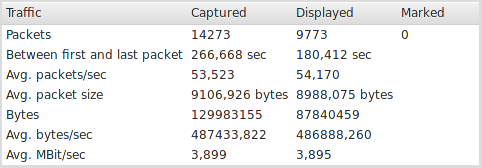
\includegraphics[scale=0.7]{vncppwifi.png}
\end{flushleft}
\caption{Rendimiento Wifi VNC++}
\end{figure}

RealVNC:
\begin{figure}[h]
\begin{flushleft}
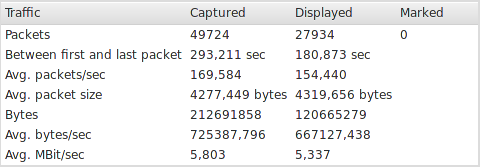
\includegraphics[scale=0.7]{realvncwifi.png}
\end{flushleft}
\caption{Rendimiento Wifi RealVNC}
\end{figure}

AndroidVNC:
\begin{figure}[h]
\begin{flushleft}
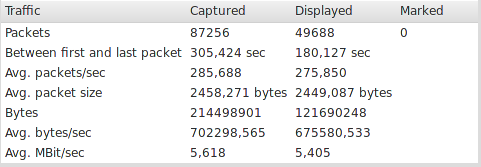
\includegraphics[scale=0.7]{androidvncwifi.png}
\end{flushleft}
\caption{Rendimiento Wifi AndroidVNC}
\end{figure}
\newpage
MultiVNC:
\begin{figure}[h]
\begin{flushleft}
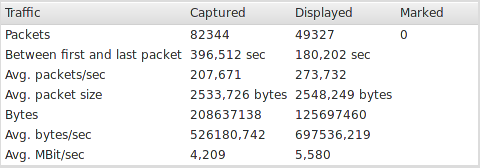
\includegraphics[scale=0.7]{multivncwifi.png}
\end{flushleft}
\caption{Rendimiento Wifi MultiVNC}
\end{figure}

Como se puede observar, los resultados de RealVNC, AndroidVNC y MultiVNC son muy parejos, esto es debido principalmente a que todos ellos utilizan la codificación para la imagen ZRLE. Sin embargo los resultados de VNC++ son muy distintos, debido a que usa Tight.\\

En primer lugar se puede observar que tanto AndroidVNC como MultiVNC tienen un tamaño medio de paquetes muy parecido, mientras que los de RealVNC son aproximadamente el doble, y a su vez, los de VNC++ el doble.\\

Por otro lado, encontramos que el promedio de Mbit/sec de RealVNC, AndroidVNC y MultiVNC es muy parecido pero el de VNC++ es significativamente inferior. Esto se debe a la codificación de la imagen, como ya dijimos anteriormente, la codificación usada por VNC++ es Tight. Esto provoca, al procesar previamente la imagen, que el uso de la red sea inferior.\\

De estos resultados se pueden concluir principalmente dos cosas:
\begin{itemize}
\item Por un lado, que debido a uso inferior de la red, VNC++ funcionaría mejor en entornos de poca conexión.
\item Y por el otro, que debido a que los paquetes son más grandes, VNC++ respondería peor a la perdida de paquetes, ya que si se pierde un paquete la información a reenviar es superior.
\end{itemize}
\newpage
\textbf{3G:}\\

VNC++:
\begin{figure}[h]
\begin{flushleft}
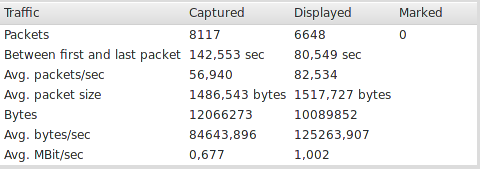
\includegraphics[scale=0.7]{vncpp3g.png}
\end{flushleft}
\caption{Rendimiento 3G VNC++}
\end{figure}

RealVNC:
\begin{figure}[h]
\begin{flushleft}
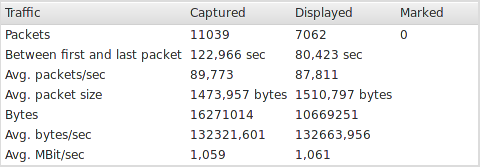
\includegraphics[scale=0.7]{realvnc3g.png}
\end{flushleft}
\caption{Rendimiento 3G RealVNC}
\end{figure}

AndroidVNC:
\begin{figure}[h]
\begin{flushleft}
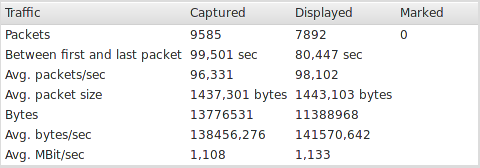
\includegraphics[scale=0.7]{androidvnc3g.png}
\end{flushleft}
\caption{Rendimiento 3G AndroidVNC}
\end{figure}
\newpage
MultiVNC:
\begin{figure}[h]
\begin{flushleft}
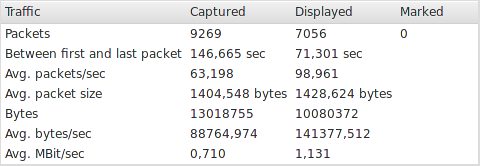
\includegraphics[scale=0.7]{multivnc3g.png}
\end{flushleft}
\caption{Rendimiento 3G MultiVNC}
\end{figure}

Como se puede observar los valores con una conexión 3G son muy parecidos, ello es debido a como funciona la propia conexión y sus limitaciones. Así pues se puede concluir que el rendimiento en entornos de 3G de las aplicaciones es equivalente.


\appendix
\clearpage % o \cleardoublepage
\addappheadtotoc
\appendixpage

\chapter{Ap\'encide}
Aquí se presenta una pequeña descripción de cómo se usa la aplicación. Este texto de ayuda se puede ver también desde la propia aplicación accediendo al menú en la ventana principal. Se encuentra tanto en español como inglés, al igual que todos los diálogos y texto de los botones. Es el propio sistema Android, en base al idioma seleccionado por defecto en el sistema operativo, el que selecciona el idioma a mostrar. En caso de no disponer del idioma correspondiente al del sistema, por defecto se mostrarán los textos en inglés.
\section{Página de ayuda de VNC++}
\subsection{Manejo principal}
Para crear una nueva conexión pulse el icono ``+'' en la barra superior de Acción (Ver Figura A.1). Una vez dentro, es necesario especificar la IP del servidor, así como un nombre de identificación de la conexión. El puerto por defecto es el 5900, pudiéndose cambiar, así como la contraseña, pudiéndose dejar en blanco si no se necesita.
\begin{figure}[h]
\hfill
\begin{minipage}[t]{.45\textwidth}
\begin{center}
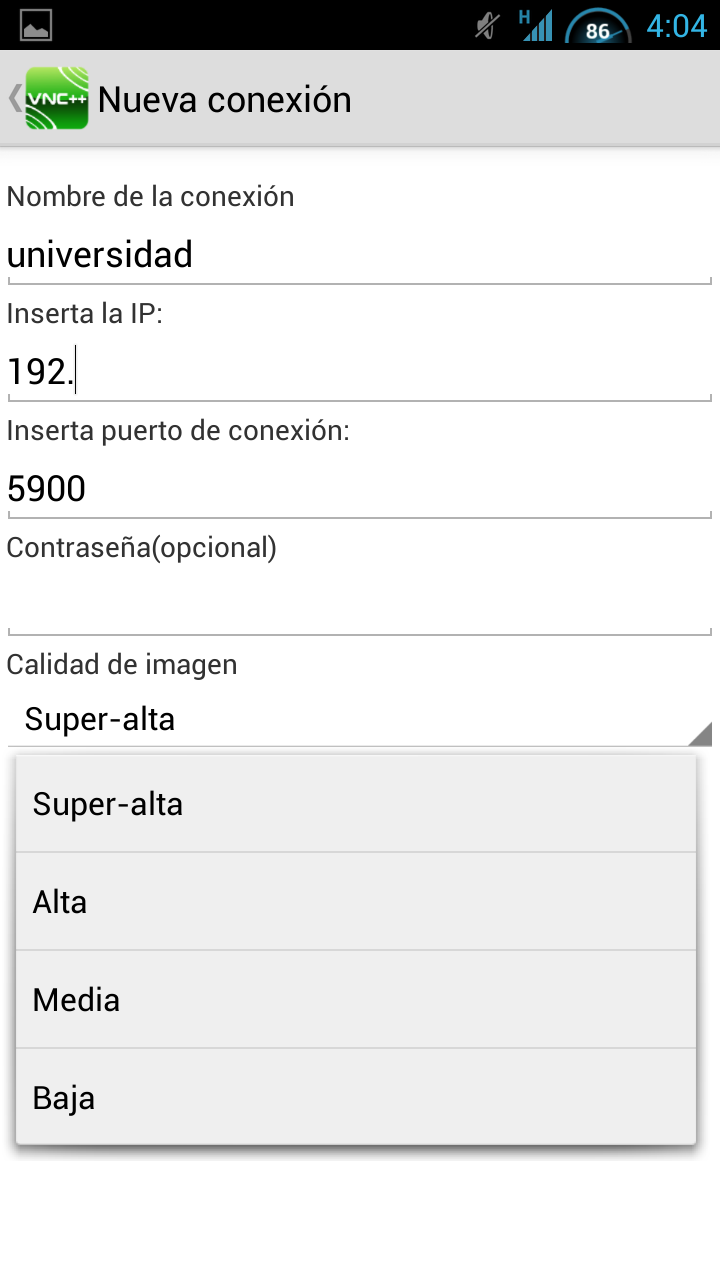
\includegraphics[scale=0.19]{Screenshot_2013-06-14-04-04-46.png}
\caption{Nueva conexión}
\end{center}
\end{minipage}
\hfill
\begin{minipage}[t]{.45\textwidth}
\begin{center}
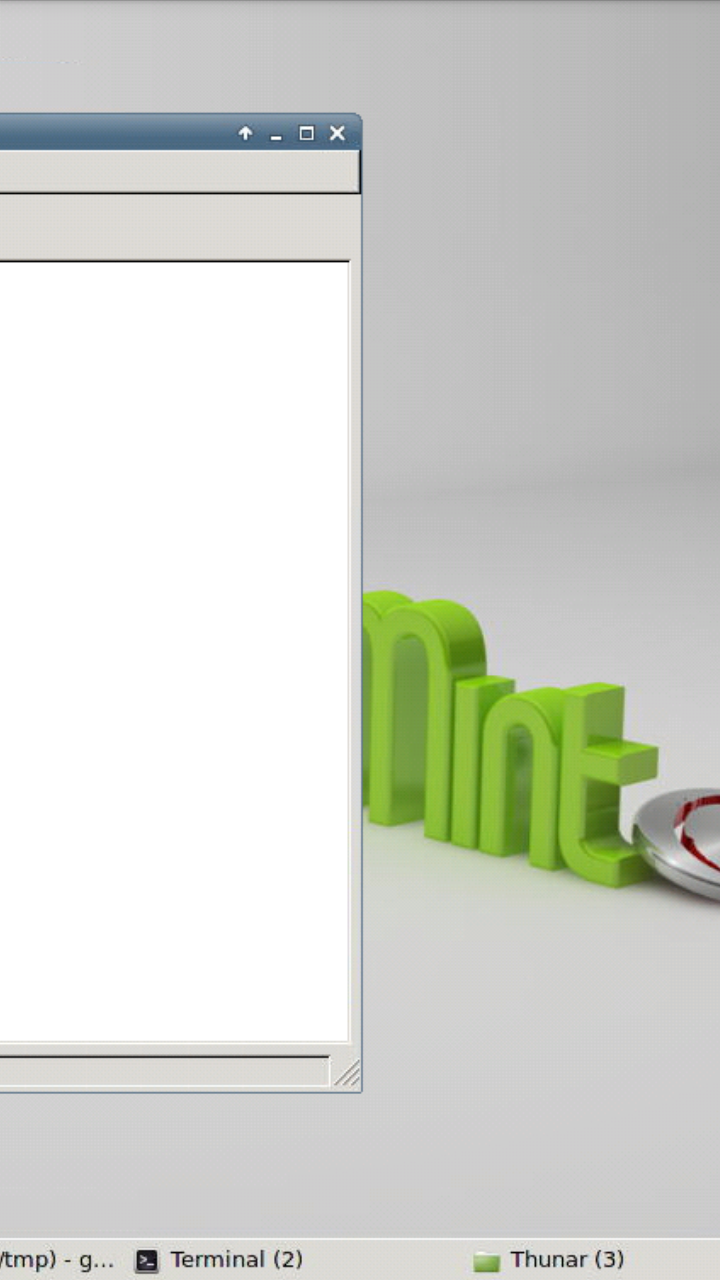
\includegraphics[scale=0.19]{Screenshot_2013-06-19-16-37-43.png}
\caption{Vista del escritorio}
\end{center}
\end{minipage}
\hfill
\end{figure}
\newpage

El desplegable de calidades sirve para indicar la calidad de la imagen. Se puede elegir entre calidad super-alta, alta, media o baja, según el tipo de conexión del usuario ya sea más lenta o rápida, o simplemente por necesidad de cierta calidad de imagen.\\

En el botón desplegable de opciones en la actividad principal se puede acceder a tres submenús:
\begin{itemize}
\item La opción de Configuración: permite, a través de dos switches de selección, marcar si se recuerda o no la opción de confirmar salida, así como ocultar el cursor o no (Ver Figura A.3).
\item Manual de uso parecido al que se está narrando (Ver Figura A.4).
\item Sección ``Acerca de'' donde se reflejan los creadores de la aplicación, así como el tipo de licencia y las librerías usadas (Ver Figura A.8).
\end{itemize}

\begin{figure}[h]
\hfill
\begin{minipage}[t]{.45\textwidth}
\begin{center}
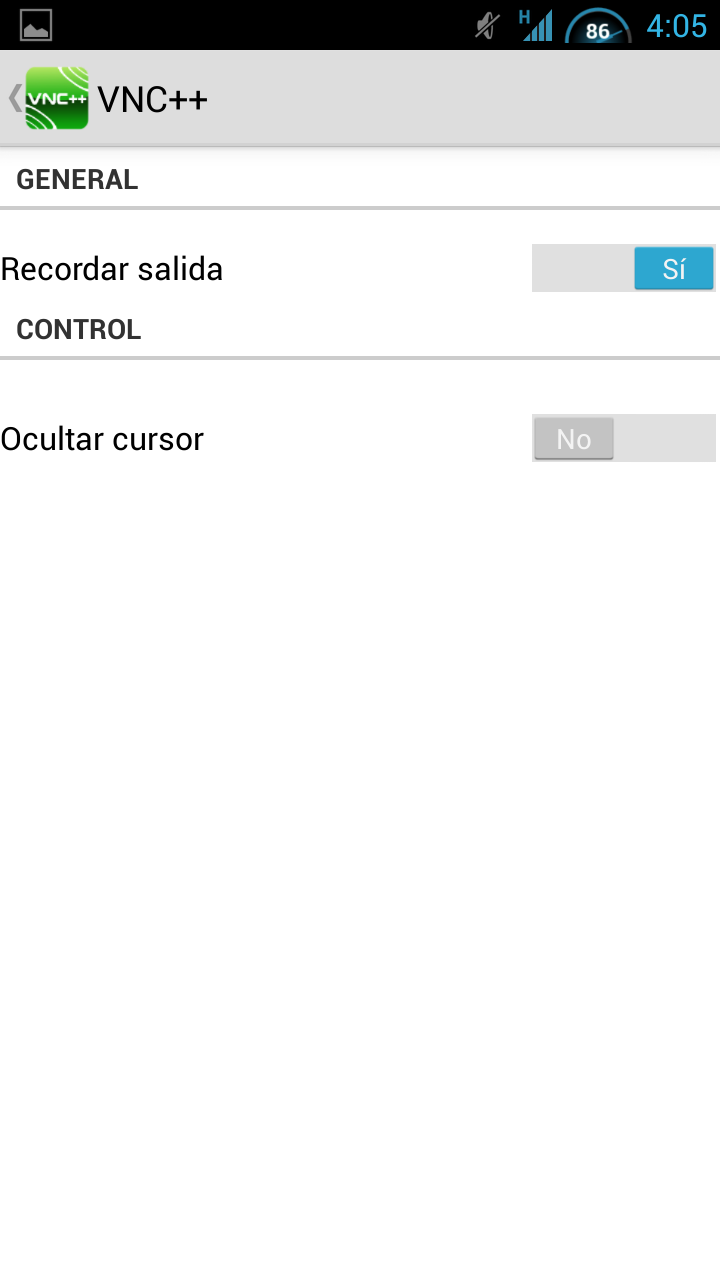
\includegraphics[scale=0.2]{Screenshot_2013-06-14-04-05-03.png}
\caption{Configuración}
\end{center}
\end{minipage}
\hfill
\begin{minipage}[t]{.45\textwidth}
\begin{center}
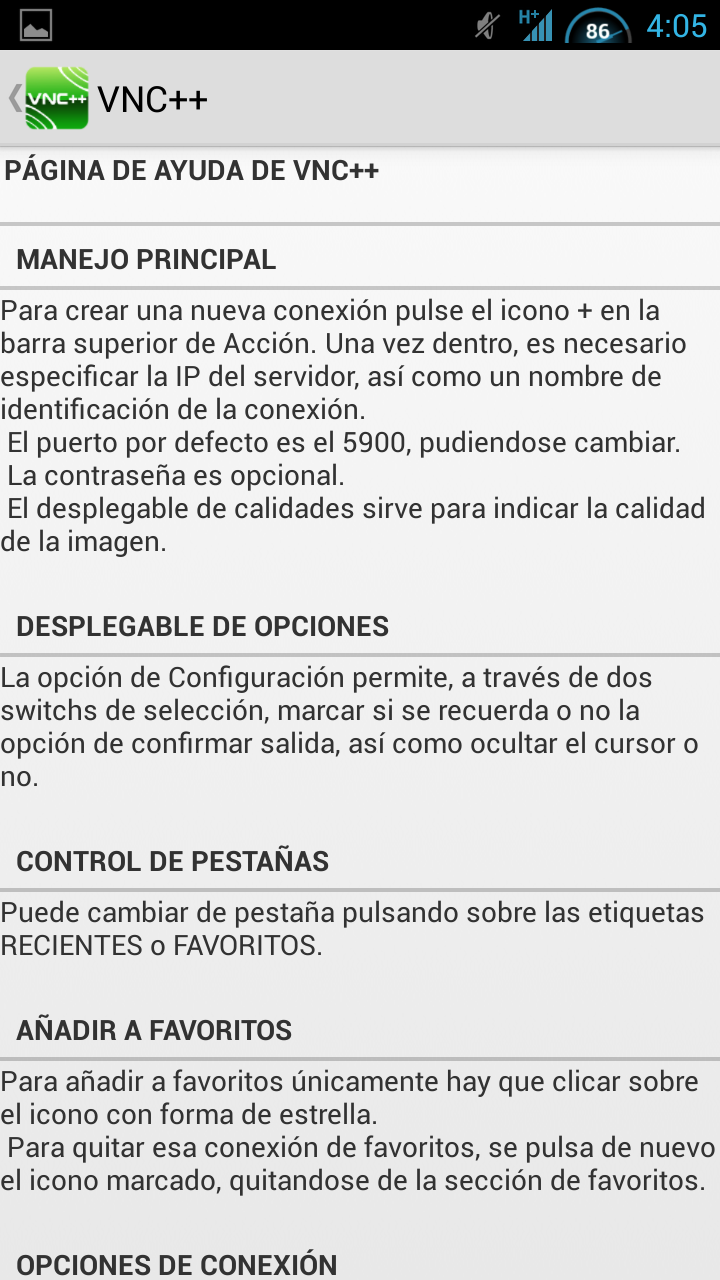
\includegraphics[scale=0.2]{Screenshot_2013-06-14-04-05-52.png}
\caption{Manual de uso}
\end{center}
\end{minipage}
\hfill
\end{figure}

\subsection{Control de pestañas}
Se puede cambiar de pestaña pulsando sobre las etiquetas RECIENTES o FAVORITOS, y así ver las distintas conexiones creadas (Ver Figura A.5).
\subsection{Añadir a favoritos}
Para añadir a favoritos únicamente hay que clicar sobre el icono con forma de estrella (Ver Figura A.5).\\

Para quitar esa conexión de favoritos, se pulsa de nuevo el icono marcado, quitándose de la sección de favoritos.
\subsection{Opciones de conexión}
Al pulsar sobre una conexión de la lista, se presenta un menú de opciones. Desde ahí se puede conectar, mostrar la información de la conexión, editar y eliminar dicha conexión. También se puede conectar pulsando el icono de la derecha con forma de flecha.

\subsection{Opciones de edición}
Se podrá modificar cualquier valor previo de la conexión, a excepción del identificador elegido, del mismo modo que se crea una nueva conexión.
\subsection{Menú lateral}
Una vez cargada la imagen se puede acceder al menú de opciones, tanto desde el botón físico del terminal, como arrastrando desde la izquierda de la pantalla para sacar el menú lateral. Una vez ahí se puede mostrar teclado, mandar teclas, centrar imagen, mostrar una ayuda reducida  y desconectar (Ver Figura A.6).
\begin{figure}[h]
\hfill
\begin{minipage}[t]{.45\textwidth}
\begin{center}
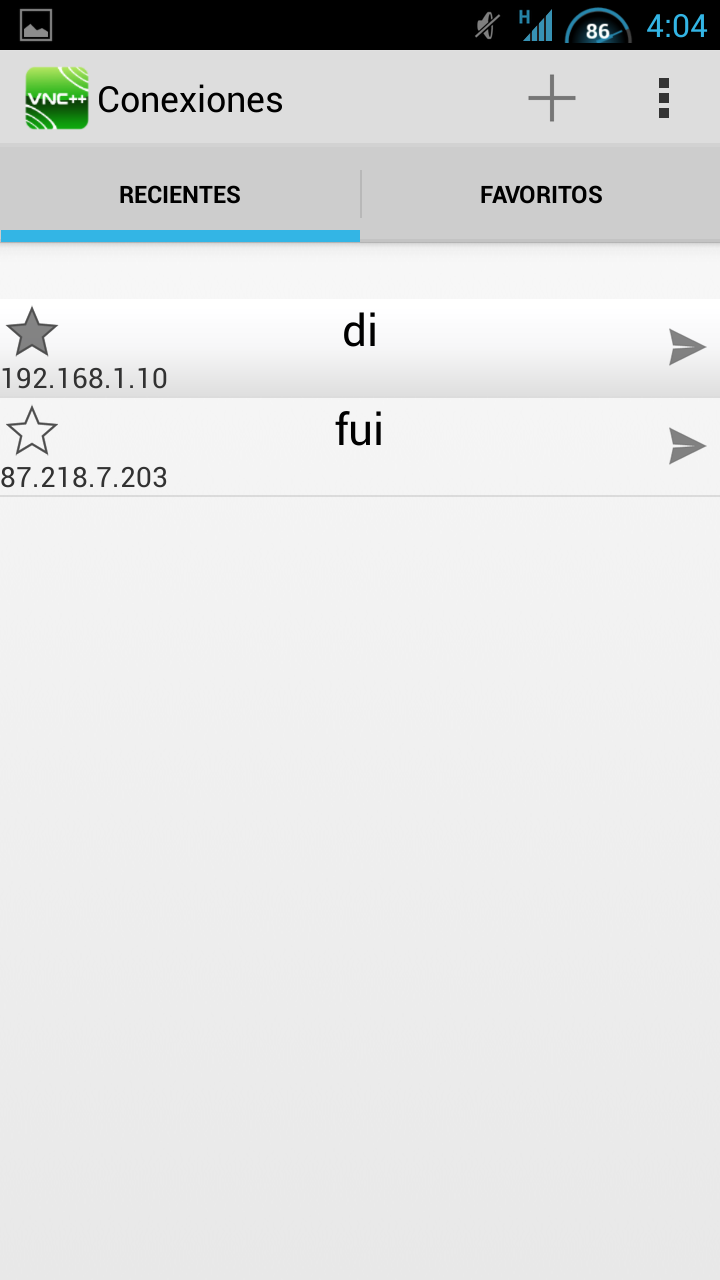
\includegraphics[scale=0.2]{Screenshot_2013-06-14-04-04-09.png}
\caption{Pestañas}
\end{center}
\end{minipage}
\hfill
\begin{minipage}[t]{.45\textwidth}
\begin{center}
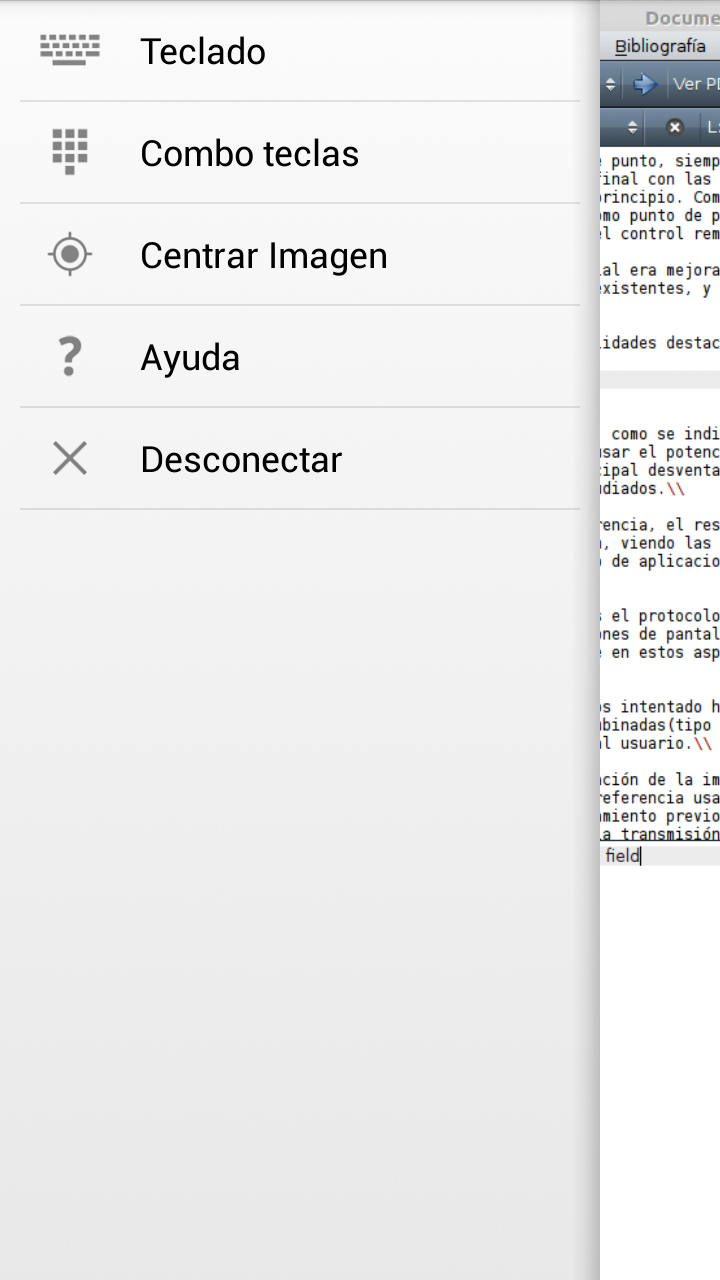
\includegraphics[scale=0.2]{Screenshot_2013-06-14-04-03-02.png}
\caption{Menú lateral}
\end{center}
\end{minipage}
\hfill
\end{figure}
\subsection{Manejo}
Para mandar evento click, simplemente haga una pulsación con el dedo.\\

Para hacer click derecho, mantenga presionado el dedo sobre la pantalla durante unos 3 segundos.\\

Para hacer zoom, coloque un dedo sobre la pantalla, mientras con otro dedo aleje o acerque del primer dedo, a modo de pinza.
\subsection{Envío de teclas especiales}
Para mandar eventos ctrl, alt, supr, shift, basta con seleccionar la tecla ``Combo teclas'', y en la ventana emergente seleccionar las teclas que se quieran enviar (Ver Figura A.7).
\begin{figure}[h]
\hfill
\begin{minipage}[t]{.45\textwidth}
\begin{center}
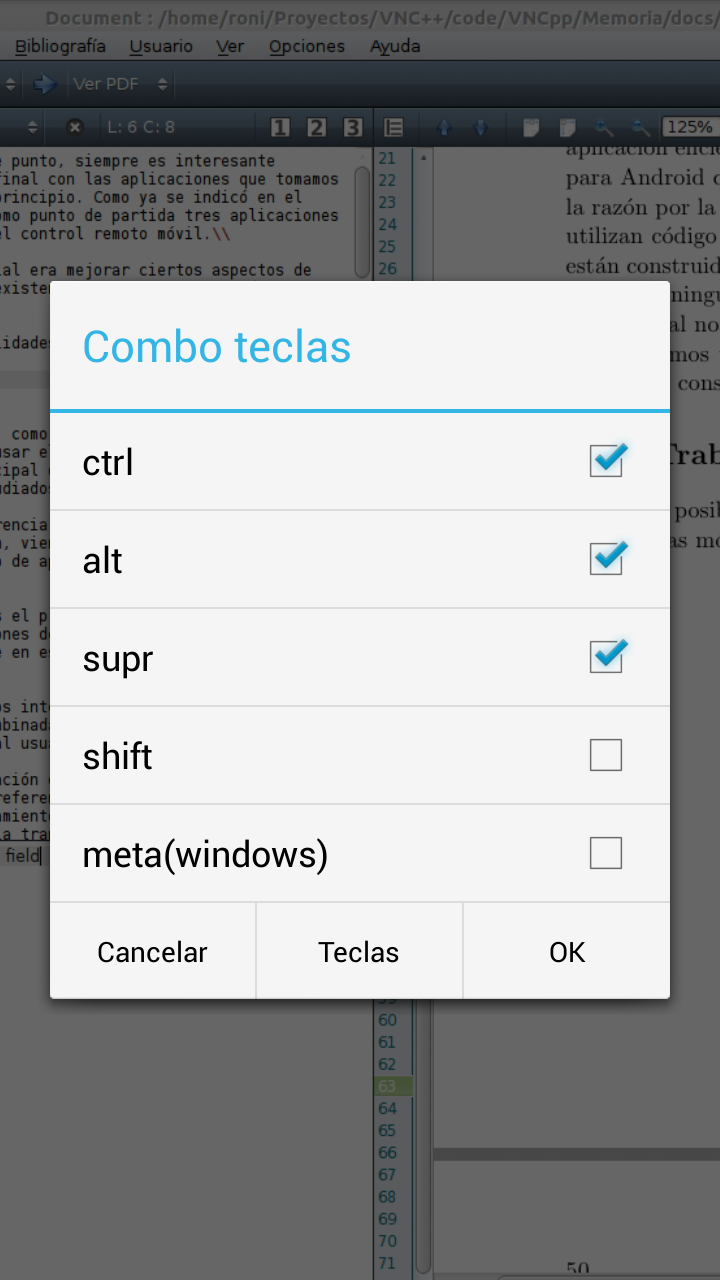
\includegraphics[scale=0.2]{Screenshot_2013-06-14-04-03-19.png}
\caption{Teclas especiales}
\end{center}
\end{minipage}
\hfill
\begin{minipage}[t]{.45\textwidth}
\begin{center}
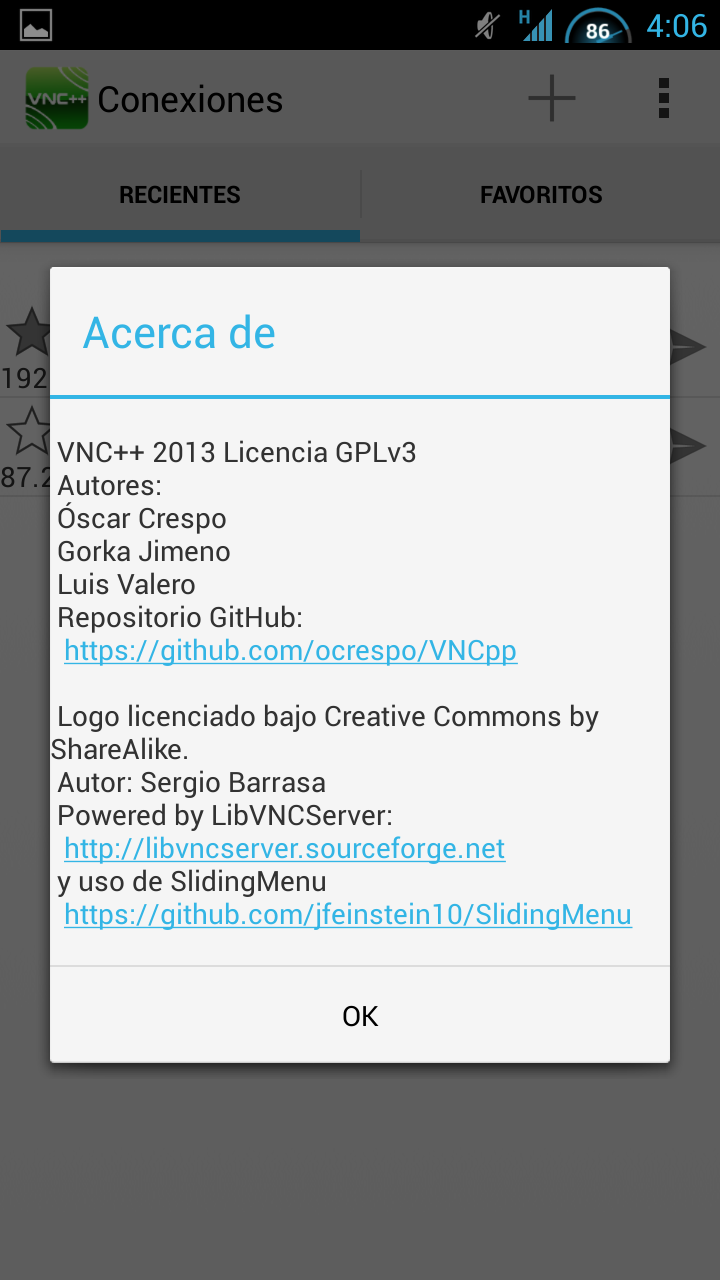
\includegraphics[scale=0.2]{Screenshot_2013-06-14-04-06-07.png}
\caption{Acerca de}
\end{center}
\end{minipage}
\hfill
\end{figure}

Las teclas función (F1, F2, etc) y el resto de letras, se pueden seleccionar desde el botón central ``Teclas''.


\end{otherlanguage}

\end{document}